% -*- TeX -*- -*- Soft -*-
%Daemon> filter=err+warn
%Daemon> custom_args="-synctex=1"
%Daemon> ini=pdflatex

\documentclass{article}
\usepackage{lscape}
\usepackage{amsmath, amsthm, amssymb}
\usepackage{a4wide}
\usepackage{gamesem}
\usepackage{pst-tree}
\usepackage{enumitem}
\usepackage{pstring}
\usepackage{xspace}
\usepackage{todonotes}
\usepackage{amsmath,amssymb,amsthm}
\usepackage{bcprules}
\usepackage{algorithm}
\usepackage{algorithmic}
\usepackage{geometry}
\usepackage{pdflscape}
%\usepackage{paralist}

\theoremstyle{definition}
\newtheorem{definition}{Definition}[section]
\newtheorem{property}{Property}[section]
\newtheorem{proposition}{Proposition}[section]
\newtheorem{remark}{Remark}[section]
\newtheorem{theorem}{Theorem}[section]
\newtheorem{conjecture}{Conjecture}[section]
\newtheorem{example}{Example}[section]
\newtheorem{observation}{Observation}[section]

% Change the numbering used for Algorithms
\renewcommand*{\thealgorithm}{\Alph{algorithm}}

\renewcommand{\algorithmicrequire}{\textbf{Input:}}
\renewcommand{\algorithmicensure}{\textbf{Output:}}


\newcommand\Nodes{N}% set of nodes
\newcommand\NodesVar{N_{\sf var}}% set of nodes
\newcommand\NodesLmd{N_\lambda}% set of nodes

\newcommand{\ghostlmd}{{\lambda\!\!\lambda}}
\newcommand{\ghostvar}{\theta}

\newcommand{\affine}{{\sf aff}}
\newcommand{\normalizing}{{\sf norm}}
\newcommand{\branching}{{\sf branch}}

\newcommand\travsetshort{\mathcal{T}\!r}
%\newcommand{\travsetaffine}{{\travset^\affine}}
\newcommand{\travsetbr}{{\travset^\branching}}
\newcommand{\travsetnorm}{\travset^\normalizing}

% for succinctness we omit ULC for the symbol representing
% set of traversals of ULC
% (this is not ambiguous since ULC and STLC are shown to coincide in this paper)
\newcommand{\travulc}{\travset}
\newcommand{\travstlc}{{\travset_{\sf STLC}}}


\newcommand{\child}{{\small \sf Ch}} % unique child of a node

\newcommand{\rulefont}[1]{\mathbf{\sf #1}}

\def\coresymbol{\pi} % function returning the core of a traversal
\newcommand{\core}[1]{\coresymbol(#1)} % core of a traversal

\newcommand{\enables}{\vdash} %enabling relation
\newcommand{\ctree}{CT} %computation tree

\newcommand{\NodeHjByRoot}{\Nodes^{\enables^*}} % set of nodes hereditarily justified by the root

\newcommand\pathset{{\mathcal{P}aths}} % set of paths in the comp tree
\newcommand\arth{\textsf{arth}} % arity threshold

\renewcommand\ie{{\it i.e.\@\xspace}}
\renewcommand\eg{{\it e.g.\@\xspace}}

\def\justseqset{\mathcal{J}}
\def\istraversal{\models}

\author{William Blum}
\title{Imaginary Traversals and Leftmost Linear Reduction [Draft]}

\begin{document}
\maketitle
\begin{abstract}
We introduce a method to normalize untyped lambda terms, when the normal-form exists, by combining the theory of traversals, a term-tree traversing techniques inspired from Game Semantics \cite{Ong2006,BlumPhd}, and judicious use of the eta-conversion rule of the lambda calculus.

Little modifications to the traversal theory of the simply-typed lambda calculus \cite{BlumPhd} is needed. A notable improvement is that eta-long transformation is unnecessary: we traverse the original unmodified term tree. Blindly applying the original traversal rules on untyped terms, which do not have a (finite) eta-long form, causes traversals to get `stuck' when an application operand is lacking; whereas in a typed setting, eta-long transform ensures that application operands necessarily exist. Relaxing this structural requirement altogether induces the notion of ``imaginary'' nodes: those are nodes that would exist
 if the subterm with the missing operand were to be eta-expanded. This allows the traversal to proceed.

We show how, by bounding the non-determinism of the free variable rule, one can effectively compute a subset of traversals that characterizes the set of paths in the beta-normal form of the term. This yields a normalization algorithm for untyped terms with a normal form.

Finally we define \emph{leftmost linear reduction} as a generalization of the head linear reduction of Danos-Regnier and show that the traversals theory implements it, which prove correctness of the normalization procedure.
\end{abstract}

\section{Background}

Traversals were originally introduced in the context of higher-order recursion schemes \cite{Ong2006} used as generator of order-$0$ structures such as trees.
The notion was then extended to the more general setting of simply-typed languages and, in particular, to the simply-typed lambda calculus \cite{BlumPhd}, where the non-deterministic rule \rulenamet{IVar} is introduced to account for the presence of free variables. The relationship with Game Semantics is well understood in the typed setting: the set of traversals is in bijection with (the plays of) the interaction game denotation of a term, further the \emph{core projection} operation yields a bijection between the standard game denotation and its standard innocent game denotation (Theorem \ref{thm:gamesem_correspondence_stlc}). This correspondence yields a method to evaluate beta-redexes of a simply-typed lambda term without performing the traditional $\beta$-reduction \cite{danos-head,BlumPhd,BlumGalop2008, Blum-LocalBeta2008}.

In this paper we show how the game-semantic traversals of STLC \cite{BlumPhd} naturally extend to ULC, and thus yield a method to normalize untyped lambda terms. In the absence of types, eta-long expansion is simply not an option: it would yield an infinite term. We thus opt instead for a more reasonable option: \emph{on-demand eta-expansion}. The idea stems from the following observation: attempting to apply the original STLC traversal rules on an untyped lambda term can lead to situations where the traversal gets ``stuck''. This happens when a sub-term in operator position has an insufficient number of operands to be able to resolve a parameter. For example, STLC traversals would get stuck when trying to resolved the ``$y$ argument'' of $f$ in term $(\lambda f.f)(\lambda y.y)$. The absence of $\eta$-long transform of the term is a notable difference with the traversals for recursion scheme \cite{Ong2006} or the simply-typed lambda calculus \cite{BlumPhd}. This simplifies the presentation as the traversed tree is just a direct representation of the original, unmodified, lambda term.

This adaptation of the game-semantic traversals to the untyped setting has several new ingredients that we will detail in the rest of the paper:
\begin{itemize}
\item  The `lambda' and `variable' rules are augmented to support eta-expansion.
 \item Eta-expansion is performed `on-the-fly` at each point where the traditional STLC traversal would normally get stuck: whenever there is insufficiently many operands in an application to continue traversing the term.
\item The concept of ``ghost'' nodes is introduced: those are are imaginary tree nodes that progressively appear as eta-expansion is performed on the sub-terms.
\item The term tree itself does not get modified during eta-expansion. Ghost nodes are only added to the traversal and are only ``visible'' in the context where they get introduced.
\item The rule used to model free variables is constrained by a quantity called the \emph{arity threshold}. This quantity, calculated in linear time from the traversal itself, limits the non-deterministic branching factor of the rule. This guarantees that the normalization procedure terminates when the beta-normal form exists.
\end{itemize}

Normalization can then be implemented by enumerating traversals. Although the set of all traversals can be infinite, we show that for the sake of normalization, it is sufficient to consider sufficiently enough traversals to ``cover'' all paths of the tree representation of the beta-normal form.

The normalization algorithm presented in this paper was implemented in the HOG tool \cite{Blum-HogTool}. The last section of the paper provides some examples of terms normalized with the algorithm.

\subsection{Related work}

\subsubsection{Head linear reduction}
In 2004, Danos and Regnier showed the connection between Game Semantics and \emph{head linear reduction}. The various notions of traversals discussed in this paper, including Berezun-Jones, are all essentially methods based on evaluating the head linear reduction sequence of a lambda term. Traversals start by performing a depth-first search to locate the \emph{head occurrence} of the \emph{hoc redex}. They implement linear substitution by ``jumping'' to the node in the tree that represents the term to be substituted for the head occurrence. At this point the traversal continues as if the head occurrence in the tree was replaced by the subtree representing the argument of the redex. Since all the terms obtained in the head linear reduction sequence are made of sub-terms of the original term, there is no need for environments or closure to evaluate the beta-redex. Instead those can be replaced by some pointer mechanism to capture a given context.

Despite the connection established in this 2004 paper, it is not explicitely shown how the head linear reduction helps normalize a term. The \emph{Pointer Abstract Machine} introduced in the same paper, for instance, yields what they call ``\emph{quasi-head normal form (qhn)}'' of the term, not the normal form itself. The resulting \emph{qhn} still needs to be first reduced to head normal form (using head reduction) and then normalized by appealing to the standard $\lambda$-calculus theory that tells us that head reduction terminates.
In this paper we generalize this notion to \emph{leftmost linear reduction}, a strategy that recrusively applies head linear reduction very much like how the standard reduction recursively applies head reduction. We show how \emph{imaginary traversals} introduced in the present paper effectively implement the leftmost linear reduction, which proves soundness of the traversal normalization procedure.

\subsubsection{Traversal of STLC}

In \cite{BlumPhd} we extended the theory of traversals to the simply-typed lambda calculus by introducing the new traversal rule \rulenamet{IVar} to model free variables present in lambda terms. (Such rule is not needed in the original presentation of traversals because higher-order recursion schemes are necessarily closed terms of ground type\cite{Ong2006}.) We then formalized the correspondence between the theory of traversals and Game semantics by establishing a bijection between traversals and the game denotation of a term. The (fairly technical) proof relies on several key ingredients \cite{BlumPhd}:
\begin{description}
  \item[Free variables] The introduction of the traversal rule \rulenamet{IVar} modeling  free variables of the lambda calculus. (In the original traversal setting, higher-order recursion schemes being necessarily closed and of ground type, such rule is not needed \cite{Ong2006});
  \item[Interaction Game Semantics] Traversals do not directly correspond to the standard game denotation. Instead they correspond to a more verbose game denotation that preserves all the internal moves played while composing the strategy denoting its subterms, whereas the standard game denotation hides those internal moves;
  \item[Traversal core] Various operations and transformations on traversals need to be introduced to prove the correspondence. In particular the \emph{projection with respect to the root of the tree} which gives the ``core'' of a traversal.
\end{description}

 This correspondence with Game Semantics yields a method to reduce beta-redexes in simply-typed lambda-terms. This normalization procedure was studied in \cite{BlumPhd,BlumGalop2008,Blum-HogTool,Ong-NormByTrav2015} and implemented in the HOG tool\cite{BlumGalop2008, BlumPhd}. We recall these results in section \ref{sec:traversal_correspondence_stlc}.

The work presented in the present paper can be viewed as a generalization of this work to the untyped case. Proposition \ref{prop:ulc_and_stlc_trav_coincide} shows that the two definition coincide for simply-typed terms.
A notable difference, however, is that the normalization procedure introduced here produces the beta-normal form of the term rather than its beta-eta-long normal form. Furthermore, we proof soundness without appealing to Game Semantics.

\subsubsection{Berezun-Jones traversals}
Berezun and Jones  introduced the first notion of traversals for the \emph{untyped} lambda calculus (ULC) \cite{JonesBerezunLLL}. Although they took inspiration from the Game Semantic traversals of \cite{Ong2006,BlumGalop2008}, their definition is more operational in nature and does not directly related to the game denotation of a term. Starting from an operational semantics of the untyped lambda calculus they derive a normalization method that, very much like the traversal of \cite{Ong2006, BlumPhd}, proceeds by traversing some tree representation of the term.

The tree representation used in Berezun-Jones' traversals are direct abstract syntax tree representation of the lambda-term, whereas in the present setting we use a more `compressed' form where consecutive lambdas and applications are merged into a single node. On the other hand, unlike the original definition of traversals for STLC where eta-long transformation is performed prior to traversing a term, both Berezun-Jones' traversals and the traversals introduced in the present paper require no prior syntactic transformation of the lambda term.

The Berezun-Jones traversals distinctively rely on two justification pointers: each `token' of the traversal can have one \emph{binding pointer} as well as one \emph{control pointer}. They also involve the use of a boolean parameter (the `flag') associated with every token of the traversal. In contrast to Berezun-Jones, the traversals presented in this paper necessitate a single justification pointer per node occurrence.

Another notable difference is that the normalization algorithm of Berezun-Jones requires a single traversal of the term. Our normalization algorithm, however, produces one traversal for every branch in the tree representing the beta-normal form. Each branching point corresponds to some occurrence of a variable in the normal form, and each branch corresponds to one operand of the variable. One can conceivably see how such non-deterministic branching could be eliminated by adding appropriate auxiliary pointers to implement backtracking: after the first operand is evaluated, backtrack to the operator variable in the traversal and explore the remaining operands.

\subsection{Rest of the paper}

In the remaining of this paper we will introduce basic definition from the traversal theory and introduce a new notion of traversals for the untyped lambda calculus. We briefly discuss the correspondence with game models of the Untyped Lambda Calculus \cite{KerThesis} and show how they yield an algorithm to normalize untyped lambda terms. Finally, we illustrate the normalization algorithm on some examples of lambda terms.

\section{Definitions}

\subsection{Untyped lambda calculus}

We consider the set of terms $\Lambda$ of the untyped lambda calculus constructed from the following grammar:
$$\Lambda := x\ |\ (\Lambda\ \Lambda)\ |\ \lambda x. \Lambda $$
where $x$ ranges over a countable set of variable names.

For conciseness when writing lambda terms, we will abbreviate ``consecutive'' lambda abstraction $\lambda x_1 \ldots \lambda x_n . U$ for some $n\geq 0$ and term $U$ as just
$\lambda x_1 \ldots x_n . U$. If $\overline{x}$ denote the list of variables $x_1 \ldots x_n$ we will just write $\lambda \overline{x} . U$.

\subsection{Computation tree and enabling relation}

Given an untyped lambda term $M$ we define its \defname{computation tree} as the abstract syntax tree (AST) representation of the lambda term where consecutive lambda abstractions are merged into a single node labelled by the list of bound variables and with a single child, and similarly consecutive applications are represented by a single node labelled $@$ with multiple children: one for the operator and one for each application operand. Formally:
\begin{definition}[Computation tree of an untyped term]
	Let $M$ be an untyped lambda term with variable names in $\mathcal{V}$.
\begin{itemize}
\item We define the set of labels:
    $$ \mathcal{L} = \{ @ \} \union \mathcal{V} \union \{ \lambda x_1 \ldots x_n \ | \ x_1 ,\ldots, x_n \in
	\mathcal{V}, n\in\nat \}$$
\item
	The \defname{computation tree} $\ctree(M)$ is a labelled tree with labels in $\mathcal{L}$
    defined inductively on the syntax of $M$:
	\begin{eqnarray*}
		\ctree(\lambda \overline{x} . z s_1 \ldots s_m) &=& \lambda \overline{x}\; \langle\; \underline z\; \langle \ctree(s_1),\ldots,\ctree(s_m)\rangle\rangle\\
		&& \hbox {where $m\geq 0$, $z \in \mathcal{V}$}, \\
 \ctree(\lambda \overline{x} . (\lambda y.t) s_1 \ldots s_m) &=& \lambda \overline{x}\; \langle\; @ \; \langle \ctree(\lambda y.t),\ctree(s_1),\ldots,\ctree(s_m) \rangle \rangle \enspace\\
&&  \hbox{where $m\geq 1$, $y\in \mathcal{V}$}.
	\end{eqnarray*}
where the expression `$l\langle t_1, \ldots, t_m \rangle$' for $m \geq 0$ denotes a labelled tree with root labelled $l$ and $m$ ordered children trees $t_1$, \ldots, $t_m$. The underlined label $z$ represents a node label for $m>0$, and a leaf label if $m=0$.

\item We write $\Nodes$ to denote the set of nodes of the computation tree. We write $\NodesVar$ for the set of variable nodes, $\NodesLmd$ for lambda nodes, and $\Nodes_@$ for  application nodes.
    
\item For any lambda node $\alpha\in\NodesLmd$ we write $\child(\alpha)$ to denote its unique child node (either an $@$ or variable node).
\end{itemize}
\end{definition}

Note that any lambda term can indeed be written in one of the two forms above. In particular, applicative terms are handled by the case $n=0$ of the form $\lambda . N$ for some term $N$ where `$\lambda.$' is referred to as a ``dummy lambda''. This compact representation turns out to be useful to maintain alternation between lambda nodes (at odd level, counting from 1 onwards) and variable nodes (at even level).

Observe that the definition is similar to that of STLC \cite{Ong2006, BlumPhd} with the notable difference that the term does not get eta-long expanded prior to constructing the computation tree.

We define the \defname{enabling relation} $\enables$ between nodes of the computation tree as the relation associating each lambda node to all the variable nodes that it binds, the root of the tree to all the free variable nodes, and every variable and application node to each of their child node. We write $m \enables_k \alpha$ to indicate that a lambda node $\alpha$ is the $k$th child of a variable or application node $m$ for some $k\geq0$; and $\alpha \enables_k m$ to indicate that the node $m$ is labelled by the $k$th variable bound by $\alpha$ for $k\geq1$.

We define \defname{hereditarily enabling} as the reflexive transitive closure $\enables^*$ of the enabling relation, and we say that node $m$ \defname{hereditarily enables} node $n$ if $m \enables^* n$. We write $\NodeHjByRoot$ to denote the set of nodes hereditarily enabled by the root, that is the image of the tree root by the reflexive transitive closure of the enabling relation.

A consequence of the definition of the enabling relation is that every node of the tree is either hereditarily justified by the root or by some application node $@$.  Variable nodes that are hereditarily enabled by the root are called \defname{external variable nodes}, and variables hereditarily justified by an application node are called \defname{internal variable nodes}.

We defined the \defname{arity} of a node as follows: the arity of a lambda node $\lambda x_1 \cdots x_k$ for $k\geq 0$ is denoted by $|\lambda x_1 \cdots x_k|$ and is defined as $k$; the arity of a variable node $x$, denoted $|x|$ is the number of children of $x$ in the computation tree; the arity of a $@$ node is the number of its children nodes minus 1 (\ie, the number of operands in the application).

\subsection{Ghost nodes}
We extend the concept of computation tree nodes by introducing two infinite classes of ``imaginary'' nodes called \defname{ghost nodes}:
one class of ``ghost variable nodes'', denoted $\ghostvar$, and one class of ``ghost lambda nodes'', denoted $\ghostlmd$. By abuse of notation we will use $\ghostvar$ and $\ghostlmd$ to refer to individual elements of the two respective classes. In the upcoming definition of traversals, ghost nodes will be used as placeholders representing lambda nodes and variable nodes from eta-expanded subterms.

We simultaneously define ghost nodes and extend the enabling relation $\enables$ for them by induction: for every (ghost) variable or application node $m$ and for all $k>|m|$ there is a ghost lambda node $\ghostlmd$ such that $m \enables_k \ghostlmd$; for all (ghost) lambda node $\alpha$ and all $k>|\alpha|$ there is a ghost variable node $\ghostvar$ such that $\alpha \enables_k \ghostvar$. Thus, each ghost variable and ghost lambda node is uniquely defined by its enabler node (possibly itself a ghost node) and associated label $k\geq 1$.

We refer to nodes $\Nodes$ of the computation tree as \defname{structural nodes}
and $\tilde{\Nodes}$ for the extended set $\Nodes + \ghostvar + \ghostlmd$ where $\ghostvar$ and $\ghostlmd$ denote the sets of ghost nodes uniquely determined by $\Nodes$ together with the enabling relation $\enables$. Nodes in $\ghostlmd$ and $\ghostvar$ are called \defname{ghost nodes}. We write $\NodesLmd^\ghostlmd$ as a shorthand for $\NodesLmd + \ghostlmd$ and $\NodesVar^\ghostvar$ as a shorthand for $\NodesVar + \ghostvar$.

By convention ghost variables and lambda nodes are assigned arity $0$.

\subsection{Justified sequence of nodes}

A \defname{justified sequence} is a sequence of nodes from the computation tree where every node occurrence $n$ in the sequence, except the first one, has an associated link (the ``justification pointer'') pointing to some previous node occurrence $j$ in the sequence (called its ``justifier'') with an associated ``link label'' $l\geq0$, such as the justifier node enables the node pointing to it by the enabling relation $\enables$ with the corresponding label (\ie, $j \enables_l n$). Such link is represented as follows:
$$\Pstr[10pt]{ s = \cdots (j){j} \ldots (n-j,25){n} }$$

Whereas the enabling relation is \emph{statically} induced by the structure of the tree, the justification relation is defined on \emph{occurrences} of nodes for a specific justified sequence.

We define the set of justified sequences of nodes over $M$, written $\justseqset(M)$, as the justified sequences over $\tilde{\Nodes}$ (the nodes from the computation tree augmented with ghost nodes).

It is sometimes convenient to represent a justification sequence using the \defname{triplet encoding}: a sequence of triplet in $\tilde{\Nodes}\times\nat\times\nat$ where the first component gives the node with label, the second component encodes the distance between a node and its justifier in the sequence ($0$ for no pointer), and the third is the link label.

The \defname{structure} of a justified sequence is defined as the sequence of triples $\{@, V, \lambda \}\nat\times\nat$ where the first component indicates the type of each occurrence ($@$-node, variable or lambda node) and the last two encodes the justification pointers as in the triplet encoding.

Two justification sequences $s$ and $u$ over $M$ are equal, written $s=u$, if their triplet encoding are the same: their underlying sequences of nodes are identical (same node) and the associated justification pointers are identical (same justifier and same pointer label). Two sequences $s$ and $u$ over two distinct terms $M$ and $N$ are \defname{equivalent}, written $s \equiv u$ just  if they have the same structure: the types of the underlying nodes in the two sequences match each other and have the same justification pointers.

\begin{example}
We have $\Pstr[10pt]{ (l){\lambda x y} \cdot (n-l,25){x} } \equiv \Pstr[10pt]{ (l){\lambda z y} \cdot (n-l,25){z}}$. But we also have $\Pstr[10pt]{ (l){\lambda x y z w t} \cdot (n-l,25){x} } \equiv \Pstr[10pt]{ (l){\lambda x} \cdot (n-l,25){x}}$ since they have same structure $(\lambda,0)\cdot(V,1)$.
\end{example}

We write $I \cong J$ to denote two subsets $I \subseteq \justseqset(M)$ and $J \subseteq \justseqset(N)$ such that there exists an isomorphism (\ie a structure-preserving bijection) between $I$ and $J$. That is there exists a bijection $\phi : I\longrightarrow J$ such that for any $j\in J$, $j \equiv \phi(j)$.

A justified sequence verifies the \defname{alternation condition} if the first node is a lambda node and subsequent nodes occurrences alternate between (i) a variable or application node (ii) a lambda node.

We say that an occurrence of a node in a justified sequence is \defname{hereditarily justified by some other occurrence} if recursively following justification pointers starting from it leads to that other occurrence in the sequence. Because justification pointers must honor the enabling relation $\enables$ induced by the term structure, if a node occurrence $n$ is hereditarily justified by some occurrence of a node $m\in\Nodes$ then $n$ is necessarily hereditarily enabled by $m$. Further if $m$ occurs only once in the justified sequence then the occurrences hereditarily justified by $m$ are precisely the occurrences of nodes that are hereditarily \emph{enabled} by $m$.

For any justified sequence $t$ we write $t^\omega$ to denote the last occurrence in $t$. The notion of sequence prefix naturally extends to justified sequences.
For any occurrence $n$ in $t$ we write $t_{\leq n}$ for the prefix subsequence of $t$ ending at $n$, and $t_{<n}$ for the prefix ending at the occurrence immediately preceding $n$ (or the empty sequence if $n$ is the first occurrence in $t$).
%and $\jp(t)$ to denote the prefix of $t$ ending at the justifier of the last node of $t$.
 We say that $t$ is an \defname{extension} of justified sequence $u$ if $u$ is a strict prefix of $t$ sharing the same justification pointers.

We use the standard operations borrowed from Game Semantics on justified sequences \cite{Abr02}.

\begin{definition}[Projection]
Let $s$ be a justified sequence of nodes.

\begin{itemize}
\item Let $n$ be a node occurring in $s$ we write $s\filter n$ to denote the subsequence of $s$ obtained by keeping only nodes that are hereditarily justified by $n$ in $s$. We call it the \defname{projection of $s$} with respect to $n$;

 \item Let $A$ be a subset of nodes in $\Nodes$, we write $s \filter A$ to denote the subsequence of $s$ obtained by keeping only nodes that are in $A$;

 \item We will consider the subsequence $s\filter\NodeHjByRoot$ of external nodes (\ie, nodes hereditarily enabled by the root). Observe that if $r_1, \ldots r_n$, $n\geq 1$ are the occurrences of the root in $s$ then it is also given by the projection of $s$ with respect to those occurrences: $s\filter\NodeHjByRoot = s\filter r_1 \filter \ldots \filter r_n$.
\end{itemize}
\end{definition}

The P-view of a justified sequence is the sub-sequence obtained by reading the sequence backwards 
and following the justification pointer every other node: (i) if the node being read is a variable node then keep that node and follow its justification pointer (\ie, skip all the occurrences ``underneath that pointer'') (ii) if the node is a lambda node then keep that node and move to the preceding node. Formally:
\begin{definition}[Views]
\label{def:views}
The P-view of a justified sequence $s$, denoted $\pview{s}$ is defined recursively  as follows
$$\begin{array}{rcll}
 \pview{\epsilon} &=&  \epsilon \\
 \pview{s \cdot n }  &=&  \pview{s} \cdot n
    & \mbox{if $n$ is a variable or $@$ node;}
    \\
 \pview{\Pstr[10pt]{ s \cdot (m){m} \ldots (lmd-m,25){n}}} &=&
        \Pstr{ \pview{s} \cdot (m2){m} \cdot (lmd2-m2,60){n} }
    & \mbox{if $n$ is a lambda node;}
    \\
 \pview{s \cdot n }  &=&  n & \mbox{if $n$ is a lambda node with no pointer.}
\end{array}$$
The O-view, denoted $\oview{s}$, is defined as the dual of the P-view:
$$\begin{array}{rcll}
 \oview{\epsilon} &=&  \epsilon \\
 \oview{s \cdot n }  &=&  \oview{s} \cdot n
    & \mbox{if $n$ is an $\lambda$-node;}
    \\
 \oview{\Pstr[10pt]{s \cdot (m){m} \cdot \ldots \cdot (x-m,30){n}}} &=&
    \Pstr{ \oview{s} \cdot (m2){m} \cdot (n2-m2,60){n} }
    & \mbox{if $n$ is a variable node;}
    \\
 \oview{s \cdot n }  &=&  n
    & \mbox{if $n$ is an $@$ node.}
\end{array}$$
\end{definition}

Given two node occurrences occurrence $n$ and $m$ in a justified sequence $s$, we say that $n$ is \defname{visible at} $m$ just if $n$ occurs in the P-view $\pview{s_{\leq m}}$.

\paragraph{Justified paths of the term tree}

We will consider paths of a term tree as a set of justified sequences. For any term $M$ we define the \defname{set of justified paths} $\pathset(M)$ as the set of justified sequences in $\justseqset(M)$ whose underlying sequences of nodes are paths in the labelled-tree $\ctree(M)$ with associated justification pointers induced by the enabling relation: occurrence of bound variable nodes are justified by their binder node with link label determined by the variable index in the binding node; free variables are justified by the root (the first node in the sequence) with label index determine by the free variable index; and lambda nodes are justified by their parent (the immediate predecessor in the sequence) with label index given by the child index.

This notion is well defined because a variable binder necessarily occurs in the path from it to the root.
\begin{property}[Path characterization]
\label{prop:tree_path_charact}
(i) An untyped term $M$ is uniquely determined by the subset of maximal justified paths of $\pathset$.
(ii) Further $M$ is uniquely determined, up to $\alpha$-conversion, by the \emph{structure} (\ie, node types and pointers) of the maximal justified paths in $\pathset$.
\end{property}
\begin{proof}
(i) follows from the fact that computation trees are in one-to-one correspondence with the standard tree representation of a lambda term, and because $\pathset(M)$ is prefix-closed it's uniquely determined by its maximal elements. (ii) is due to the fact that variables names are uniquely determined by the justification pointers and their associated label index.
\end{proof}

\begin{example}
  $\pathset((\lambda x. x y) (\lambda z .z))$ is the prefix closure of 
  $\{
  \Pstr{ (r){\lambda} (at){@} (lx-at,30:0){\lambda x} (x-lx,30:1){x} (l2-x,30:1){\lambda} (y-r,40:1){y} },
  \Pstr{ (r){\lambda} (at){@} (lz-at,35:1){\lambda z} (z-lz,35:1){z}}
  \}$.
\end{example}


\section{Traversals}

\subsection{Definition and properties}

\begin{definition}[ULC traversals]
The set of \defname{traversals} of an untyped lambda term $M$, denoted $\travulc(M)$, abbreviated $\travulc$ when the term is clear from context, is the set of justified sequences of nodes over $M$ recursively defined by the rules of Table \ref{tab:trav_rules}.

A traversal that does not have any extension is a \defname{maximal traversal}.
\end{definition}

\begin{FramedTable}
\noindent {\bf PROGRAM -- Structural rules}
\begin{itemize}[]
    \item\rulenamet{Root} The singleton sequence $r$ is in $\travulc$ where $r$ is the root of the tree.

    \item \rulenamet{App} If $t \cdot @$ is a traversal then so is \Pstr[0.4cm]{t \cdot (at) @  \cdot (a-at,40:0) \alpha} where $\alpha\in\NodesLmd$ is $@$'s $0$th child $\lambda$-node.

    \item \rulenamet{Lam} If $t \cdot \alpha$ is a traversal where $\alpha\in\NodesLmd$ then so is$t \cdot \alpha \cdot n$ where $n$ denotes $\alpha$'s unique child. Furthermore:
        \begin{compactitem}
            \item \rulenamet{Lam^@} If $n$ is an $@$-node then it has no justifier,
            \item \rulenamet{Lam^{\sf var}} If $n$ is a free variable node then it points
            to the only occurrence of the root in
            $\pview{t \cdot \alpha}$. If $n$ is a bound variable then it points to the only occurrence of its binder in $\pview{t\cdot \alpha}$.
        \end{compactitem}

    \item \rulenamet{Lam^\ghostlmd} If
  $\Pstr[0.5cm]{ t \cdot(alpha){\alpha} \cdot
(n){n} \cdot \ldots \cdot
(gl-n,40:i){\ghostlmd} \in\travulc}$ for some prefix $t$, $\alpha \in \NodesLmd^\ghostlmd$ and $n \in\NodesVar^\ghostvar$ then
$$\Pstr[0.5cm]{ t \cdot(alpha){\alpha} \cdot
(n){n}
\cdot \ldots \cdot
(gl-n,40:i){\ghostlmd}\cdot (al-alpha,40:{|\alpha| + i - |n|}){\ghostvar}
      \in\travulc}$$
\end{itemize}
\emph{\bf PROGRAM -- Copy-cat rules}
\begin{itemize}
\item \rulenamet{Var} If \Pstr[0.5cm]{t \cdot (m){m} \cdot (alpha){\alpha}
    \ldots (n-alpha,50:i){n} \in \travulc} for $i>0$, $n \in \NodesVar^\ghostvar$ hereditarily justified by an $@$-node;
     $m \in \NodesVar^\ghostvar \union \Nodes_@$; and $\alpha \in \NodesLmd^\ghostlmd$ then:
  $$\Pstr[0.5cm]{ t  \cdot
(m){m} \cdot (lx){\alpha}  \ldots (x-lx,30:i){n}
    \cdot (letai-m,40:i){\beta}
     \in\travulc}$$
\begin{description}[align=right,labelwidth=2cm]
\item[Concrete] $i \leq |m|$: $\beta\in\NodesLmd$ is the $i$th child of $m$;
\item[Eta-expanded] $i > |m|$: $\beta$ is a ghost lambda node $\ghostlmd$.
\end{description}
\end{itemize}

\emph{\bf DATA -- Input-variable rules}
\begin{itemize}
\item \rulenamet{IVar} If $t \cdot n$ is a traversal where $n \in \NodesVar^\ghostvar$ is hereditarily justified by the root. For every node $m \in \NodesVar^\ghostvar$ occurring in $\oview{t\cdot n}$
and every $i\geq1$ we have $t \cdot n \cdot \alpha \in \travulc$ with $\alpha$ pointing to $m$ with label $i$, where:
\begin{description}[align=right,labelwidth=2cm]
\item[Concrete] $i\leq|m|$: $\alpha \in \Nodes_\lambda$ is the $i$th child of $m$;
\item[Eta-expanded] $i>|m|$: $\alpha$ is a ghost lambda node $\ghostlmd$.
\end{description}
\end{itemize}


\caption{Imaginary traversals $\travulc$ of the untyped lambda calculus}
 \label{tab:trav_rules}
\end{FramedTable}

Some immediate property that can be shown by induction on the rules:
\begin{property}
   For any traversal $t$
   \begin{enumerate}
   \item $t$ verifies the alternation condition;
   \item $t\filter\NodeHjByRoot$ is a valid justified sequence (with respect to the enabling relation $\enables$) verifying the alternation condition.
   \end{enumerate}
\end{property}




\paragraph{On-the-fly expansion}
The following definition explicit the notions of \emph{on-the-fly eta-expansion} implemented by the
traversal rules \rulenamet{Var} and \rulenamet{IVar}:

\begin{definition}[On-the-fly eta-expansion]
\label{def:onthefly_etaexpansion}
Let $M$ be an untyped term.
\begin{itemize}
\item Let $n$ be a node of the tree of $M$ and $N$ denote the subterm of $M$ rooted at $n$. We write $ETA(M, n)$ to denote the term obtained by substituting
the subterm $N$ in $M$ with the term $\lambda \theta. N \theta$ for some variable $\theta$ fresh in $N$.

\item Let $M$ be an untyped term and $t$ be a \emph{finite} traversal of $M$. We define the \defname{eta-expansion of $M$ with respect to $t$}, written $M^t$, as a term obtained by eta-expanding its subterms according to the rules used to traverse $M$. It is defined by induction on the traversal rules: By convention we define $M^\epsilon = M$. Suppose $t = u \cdot n$ for some node $n$. Let $m$ denote the justifier of $n$ if it exists and $i$ denote its link label.  Consider the last rule used to traverse $t$:
\begin{equation}
M^{u \cdot n} =
\begin{cases}
    \rulename{Root} &  M^{u} \\
    \rulename{App} &  M^{u} \\
    \rulename{Lam} &  M^{u} \\
    \rulename{Lam^\ghostlmd} & M^{u} \\
    \rulename{Var} &  M^{u} \hfill \mbox{if $i \leq |m|$; } \\
                   & ETA(M^{u}, m) \hfill  \mbox{if $i > |m|$; } \\
    \rulename{IVar} &  M^{u} \hfill \mbox{if $i \leq |m|$; } \\
                   & ETA(M^{u}, m) \qquad \hfill \mbox{if $i > |m|$.}
\end{cases}
\end{equation}
\end{itemize}
\end{definition}
Observe that the tree obtained after eta-expansion with respect to $t$ contains the tree of $M$ itself, therefore paths in the tree of $M$ are also paths in the tree of $M^t$.

\begin{example}
Take $M = (\lambda u . u\ (y_1\ u)) (\lambda v . v\ y_2)$. Its computation tree is shown in Ex.~\ref{ex:missingoperand}. A valid traversal is $t = \Pstr[0.7cm]{(n0){\lambda }\ (n1){@}\ (n2-n1){\lambda u}\ (n3-n2){u}\ (n4-n1){\lambda v}\ (n5-n4){v}\ (n6-n3){\lambda }\ (n7-n0){y_1}\ (n8-n7){\lambda }\ (n9-n2){u}\ (n10-n1){\lambda v}\ (n11-n10){v}\ (n12-n9){{\ghostlmd^{1}}}\ (n13-n8){{\ghostvar^{1}}}\ (n14-n13){{\ghostlmd^{1}}}\ (n15-n12){{\ghostvar^{1}}}\ (n16-n11){\lambda }\ (n17-n0,35){y_2}\ }$. The eta expansion of $M$ with respect to $t$ is
$M^t = (\lambda u . u~(y_1~(\lambda \alpha. u (\lambda \beta.\alpha \beta))) (\lambda v . v~y_2)$.
\end{example}

\paragraph{Path-View correspondence}
We now generalize a known result from the theory of traversals for higher-order grammars \cite{Ong2006} and simply-typed lambda terms \cite[Proposition 4.29]{BlumPhd} to the untyped setting: The game-semantic concept of `Proponent view' from definition \ref{def:views} corresponds to the concept of `tree path' in the following sense:

\begin{proposition}[Path-View correspondence for ULC]
\label{prop:pathview_ulc}
Let $M$ be an untyped term and $t$ be a \emph{finite} traversal of $M$ then
$\pview{t}$ is a path (with associated justification pointers) in the computation tree of the eta-expansion of $M$ with respect to $t$.
In particular, if $t$ does not contain any ghost node then $\pview{t}$ is a path in the computation tree of $M$.
\end{proposition}
\begin{proof}
Proven by induction on the traversal rules of $t$.
\end{proof}

\begin{property}
The traversal rules are well-defined.
\end{property}
\begin{proof}
(i) Rule \rulenamet{Lam}: By Proposition \ref{prop:pathview_ulc}, the P-view is a path in the tree of the eta-expansion of $M$ with respect to $t$. But the last node of $t$ is a structural node therefore, since the eta-expanded tree contains the tree of $M$, this path is necessarily also the path to $t^\omega$ in the tree of $M$ (and thus $\pview{t}$ does not contain any ghost node, even though $t$ itself may contain ghost nodes).
 Consequently, if the last node is a variable node, its enabler necessarily occurs exactly once in the P-view.

(ii) Rule \rulenamet{Var}: In the concrete sub-case, $m$ is necessarily itself a structural node since $|m|\geq i>0$, and its $i$th child exists in $\Nodes$ since $m$ as arity greater than $i$.
\end{proof}

\paragraph{Traversal core}

We now generalize the notion of \emph{traversal core} from \cite{BlumPhd} to the imaginary traversals.
In the typed setting, the core of a traversal is the subsequence consisting of external nodes. In the untyped setting it is obtained by taking the subsequence of external nodes followed by a relabelling operation on lambda nodes.

We will consider sequence of variable names in $\mathcal{V}^*$ as stack.
For any sequence of variables $\overline{x} = x_1 \ldots x_n$, we define the stack pop operation $pop_j$, $n,j\geq0$ that removes the first $j$ elements of the sequence: $pop_j (x_1 \ldots x_n) = x_{j+1} \ldots x_n$ if $j<n$, and $pop_j (x_1 \ldots x_n) = \epsilon$ otherwise. And for any sequence $\overline{y} = y_1 \ldots y_m$, $m\geq0$ we write $\overline{x}\overline{y}$ for
$x_1 \ldots x_n y_1 \ldots y_n$, the stack obtained after pushing the variables $\overline{x}$ onto $\overline{y}$.

\begin{definition}[Core projection]
  \label{def:coreprojection}
We first define the partial function $\coresymbol \colon \travulc(M) \longrightarrow \justseqset(M)$ for traversals that do not contain any ghost occurrences then extend the notion to all traversals.
\begin{itemize}
\item For any stack $\overline{y} \in \mathcal{V}^*$ of variable names and traversal $t\in\travulc(M)$ we define $\coresymbol (t)$ by induction on $t$:
\begin{align*}
\coresymbol_{\overline{y}} \colon \travulc(M) & \longrightarrow \justseqset(M) \\
 t\cdot x &\longmapsto \coresymbol_{\epsilon}(t) \cdot x & \mbox{if } x\in \NodeHjByRoot \\
 t\cdot x &\longmapsto \coresymbol_{\overline{y}}(t) & \mbox{if } x\not\in\NodeHjByRoot \\
 t\cdot @ &\longmapsto \coresymbol_{pop_k({\overline{y}})}(t) & \mbox{where $k = |@|$} \\
 t\cdot \lambda \overline{x} & \longmapsto \coresymbol_{\epsilon}(t) \cdot \lambda \overline{x}\overline{y} & \mbox{if } \lambda \overline{x}\in \NodeHjByRoot \\
 t\cdot \lambda \overline{x} & \longmapsto \coresymbol_{\overline{x} \overline{y}}(t) & \mbox{if } \lambda \overline{x}\not\in \NodeHjByRoot \ .
\end{align*}

\item We extend $\coresymbol$ to all traversals as follows:
\begin{align*}
\coresymbol_{\overline{y}} \colon \travulc(M) & \longrightarrow \justseqset^\eta(M) \\
 t &\longmapsto \coresymbol_{\overline{y}}(\eta(t))
\end{align*}
where $\justseqset^\eta(M)$ be the union of the sets of justified sequences of nodes over eta-expansions of $M$ with respect to all possible traversals:
$$\justseqset^\eta(M) = \Union_{t\in\travulc(M)} \justseqset(M^t) \ .$$
\end{itemize}

We call $\coresymbol_\epsilon(t)$ the \defname{core} of $t$ which we abbreviate as $\core{t}$.
We define the \defname{core P-view} as $\pview{\core{t}}$, the P-view of the traversal core.

\end{definition}

The stack parameter $\overline{y}$ from the above definition represents the sequence of abstractions $\lambda \overline{y}$ and is therefore called the \defname{stack of pending lambdas}. Thus, in words, the \emph{core projection} is given by the subsequence of external nodes where each lambda node label is suffixed with the \emph{pending lambdas} of the maximal consecutive sequence of internal nodes following it.

\begin{proposition}
\label{prop:eta_expanded_trav}
Let $M$ be an untyped term and $t$ be a \emph{finite} traversal of $M$.
Let $\Nodes$ and $\Nodes_t$ denote the nodes of tree $\ctree(M)$ and $\ctree(M^t)$ respectively. Then there exists a one-to-one mapping:
$$
\eta_t : \tilde{\Nodes} \longrightarrow \tilde{\Nodes_t}
$$
with implicit \emph{element-wise pointer-preserving} extension to justified sequences $\eta_t : \mathcal{J}(M) \longrightarrow \mathcal{J}(M^t)$ such that:
\begin{enumerate}[label=(\roman*)]
  \item For any $u \in \travulc(M)$, $\eta_t(u)$ is a traversal of $M^t$.

  \item If $v$ is a \emph{finite} traversal of $M^t$ that does not contain any ghost node then there exists a traversal $u$ of $M$ (with possibly ghost nodes) such that $v = \eta_t(u)$.

  \item The restriction of $\eta_t$ to $\travset(M)$ defines a bijection with $\travset(M^t)$. Further the bijection is strong in the sense that the traversal structure (node type and pointers, but no necessarily labels) are preserved.
\end{enumerate}
\end{proposition}
\begin{proof}
The tree $\ctree(M)$ being by definition a subtree of $\ctree(M^t)$, it induces a one-to-one mapping from $\Nodes(M)$ to $\Nodes(M^t)$.
We extend it to ghost nodes by mapping ghost occurrences in $t$ to the corresponding node resulting from the eta-expansions of subterms of $M$ in $M^t$, and all other ghost nodes not occurring in $t$ to the corresponding ghost nodes in $\ctree(M^t)$. The map $\eta_t$ can be formally defined by induction on the traversal $t$, observing that in the variable rules \rulenamet{Var} and \rulenamet{IVar}, the on-the-fly eta-expansion of Definition~\ref{def:onthefly_etaexpansion} increments the arity of the justifier node $m$, therefore the corresponding structural node must exist in $M^t$.

(i) By induction on $u$. Reusing the rule used to traverse $u$ in order to traverse $v$. For the case \rulenamet{Var} and \rulenamet{IVar}, the \emph{concrete} sub-case is used instead of the \emph{eta-expanded} subcase when traversing a ghost variable that also appeared in $t$.

(ii) By induction on $v$, applying to $u$ each rule that is applied to $v$. For the case \rulenamet{Var} and \rulenamet{IVar}, if the index $i$ is greater than the arity of the node $m$ in $M$ then the lambda node from $v$ gets replaced by a ghost lambda node in $u$.

(iii) By (i) the function is well defined, it is injective by definition and by (ii) it is surjective.

\end{proof}

\begin{example}
Continuing with the example above: the following traversal obtained from $t$ is a valid traversal of $M^t$ where the occurrences corresponding to ghosts in $t$ are underlined:
$$\Pstr[0.7cm]{(n0){\lambda }~(n1){@}\ (n2-n1){\lambda u}~(n3-n2){u}~(n4-n1){\lambda v}~(n5-n4){v}\ (n6-n3){\bf \lambda}\ (n7-n0){y_1}\ (n8-n7){\bf \lambda}~(n9-n2){u}~(n10-n1){\lambda v}~(n11-n10){v}\ (n12-n9){\underline{\lambda\beta}}~(n13-n8){\underline{\alpha}}~(n14-n13){\underline{\lambda}}~(n15-n12){\underline{\beta}}\ (n16-n11){\lambda}~(n17-n0,35){y_2} }.$$
\end{example}


\subsection{Imaginary traversals subsume STLC traversals}

Traversals for simply-typed languages were previously studied in \cite{BlumPhd}.
The traversal rules defined in Table \ref{tab:trav_rules} closely match those of the simply-typed lambda calculus and PCF from \cite{BlumPhd} with some important differences:
\begin{description}
  \item[No interpreted constants] Unlike PCF, there are no interpreted constants in the present setting therefore the rule \rulenamet{Value} and \rulenamet{InputValue} from the original presentation are not needed.

  \item[No $\eta$-long expansion] In the original STLC traversals, the term is eta-long expanded prior to calculating the set of traversals. This guarantees that the operand of an application always exists in the tree.
  Imaginary traversals, on the other hand, are defined on the unmodified tree representation of the term.

  \item[On-the-fly $\eta$-expansion] In the untyped setting, eta-long expansion is an infinite process, so instead of eta-long expanding the term prior to traversing it, imaginary traversals perform eta-expansion  `on the fly'. Eta-expansion occurs in rule \rulenamet{Var} when the arity of a variable in operand position is too low to statically determine the operand of an application (case $i>|n|$). When the variable arity is high enough ($i\geq|n|$), the definition of the rule coincides with STLC and the static tree representation of the term dictates the next node to visit.

  \item[Free variables] Eta-expansion can also occur on free variables, so like for  rule \rulenamet{Var}, the input-variable rule allows for infinitely many eta-expansions ($k>0$).

  \item[Traversl core] In the typed setting, the core is  obtained by just filtering nodes with respect to the tree root. In the untyped settings, additionally, lambda nodes are relabelled.

  \item[Traversing ghost nodes] There is an additional rule \rulenamet{Lam^\ghostlmd} for the case where a traversal ends with a ghost lambda node. In the concrete sub-case, rule \rulenamet{Lam} visits the unique child node of the last lambda node in the traversal. In the eta-expanded sub-case where the last node is a ghost lambda node, there is no such child node, so we visit an imaginary one: the variable node that would be created if we were to eta-expand the sub-term under the lambda.

   The ghost placeholder $\ghostvar$ thus represents an occurrence of the $j$th variable that would be bound by lambda node $\alpha$ if the sub-term at node $\alpha$ were eta-expanded $i-|n|$ times: hence $j = |\alpha| + i - |n|$.
   (Observe that in this case we necessarily have $i>|n|$ since the $i$th child of $n$ is a ghost variable node.)
\end{description}

Let's fix a simply-typed term-in-context $\Gamma \entail M :T$, with typed-context $\Gamma$ (a set of typed variables), and simple type $T$. Its \defname{eta-long form} is defined inductively on the type $T$ and is obtained by recursively eta-expanding every subterm as many times as possible with respect to the type of the subterm \cite{Ong2006,BlumPhd}.
By abuse of language we will say that an untyped term $M$ is in eta-long form if it inhabits a simple type $T$ such that the eta-long expansion of it with respect to $T$ is $M$ itself.

The rules of the STLC traversals from \cite{BlumPhd} consist of a subset of the imaginary traversal rules of Table \ref{tab:trav_rules}.

\begin{definition}[STLC traversal \cite{BlumPhd}]
Given a simply-typed term in context $\Gamma \vdash M : T$ we write $\travstlc(\Gamma \vdash M : T)$ to denote the set of justified sequences of nodes from the tree of the \emph{eta-long form} of $M$ obtained with the rules of Table \ref{tab:trav_rules} with the exclusion of \rulenamet{Lam^\ghostlmd} and without the `Eta-expanded' sub-cases of rule \rulenamet{Var} and \rulenamet{IVar}.
\end{definition}

The above definition is well-defined:
\begin{proposition}[ULC and STLC traversals coincide]
\label{prop:ulc_and_stlc_trav_coincide}
Let $M$ be an untyped term that inhabits the simple type $T$, that is for some context $\Gamma$ we have $\Gamma \vdash M : T$. Let $\etalf{M}$ denote the \emph{eta-long normal form} with respect to $T$:
\begin{itemize}
\item[(i)] Traversals in $\travulc(\etalf{M})$ do not contain any ghost node.
\item[(ii)] $\travstlc(\Gamma \vdash M : T) = \travulc(\etalf{M})$.
\end{itemize}
\end{proposition}
\begin{proof}
(i) Because the term is eta-long expanded, the condition $i>|m|$ in the rules \rulenamet{Var} and \rulenamet{IVar} never holds while traversing the term.  This is shown by induction on the traversal rules, observing that the arity of an $@$ node is necessarily equal to the arity of the its $0$th child lambda node and that the arity of a variable node with binding index $i$ is necessarily equal to the arity of the $i$th child lambda node of its binder's parent.

(ii) By definition of $\travstlc$, the remaining traversals rules of STLC and ULC coincide, therefore the equality holds.
\end{proof}


\subsection{Property of ghost nodes}

It is helpful to think of ghost nodes as the counterpart of complex numbers sometimes used in mathematics
to prove trigonometry identities: they are introduced intermediately to perform some computation or calculation (e.g. using De Moivre's Theorem) but do not appear in the final result. Just like the imaginary number $i$ is created out of the impossibility of calculating the square root of $-1$, ghost nodes are defined from the impossibility of ``traversing'' a beta-redex of a lambda term due to an insufficient number of operands.


Ghost nodes appear in a traversal when the arity of a node is too low to continue a
structural traversal of the tree:
\begin{property}
If $\Pstr[0.5cm]{(x){x} \cdots (y-x,30:i){y}} \in \travulc$ then
$ y \in \ghostvar \union \ghostlmd \iff i > |x|.$
In particular for all $n\in\NodesVar$ and $\alpha\in\NodesLmd$:
\begin{enumerate}
\item $\Pstr[0.5cm]{(x){n} \cdots (y-x,30:i){\ghostlmd}} \in \travulc \implies i > |n|$
\item $\Pstr[0.5cm]{(x){\alpha} \cdots (y-x,30:i){\ghostvar}} \in \travulc \implies i > |n|$.
\end{enumerate}
\end{property}

\begin{definition}
We call \defname{ghost materialization} any application of a traversal rule where the last occurrence in the traversal prior to applying the rule is a ghost node ($\ghostvar$ or $\ghostlmd$), and the node traversed after applying the rule is a structural node of the tree (in $\Nodes$).
\end{definition}

\begin{remark}[\rulenamet{Var} materialization]
Observe that among all the rules defined in Table \ref{tab:trav_rules}, the rule \rulenamet{Var} is the only rule that can materialize a structural node in $\Nodes$ from a traversal ending with a ghost node. This means that after traversing ghost nodes, the only way to `come back' to structural nodes is to visit a ghost variable node $\ghostvar$ with an application of rule \rulenamet{Var} of the following form:

$$\rulename{Var}\ \  \Pstr[0.5cm]{ t \cdot(beta){\beta} \cdot
(y){y} \cdot (l){\alpha}  \ldots (t-l,30:i){\ghostvar}
    \cdot (lx-y,40:i){\lambda \overline{x}}
     \in\travulc}$$
where
\begin{itemize}
\item $y \in \NodesVar$,
\item $\lambda \overline{x} \in \NodesLmd$ is the $i$th child lambda node of $y \in \NodesVar$,
\item $\alpha$ is either a structural lambda node in $\Nodes_\lambda$ or a ghost lambda node in $\ghostlmd$,
\item $0\leq \alpha < i \leq |y|$.
\end{itemize}
\end{remark}

\subsection{Correspondence with Game semantics}
\label{sec:traversal_correspondence_stlc}

In \cite{BlumPhd} we formalized the correspondence between the theory of traversals and Game Semantics in the setting of simply-typed languages: there is a bijection between the set of traversals of $M$ and the revealed interaction game denotation of $M$. Furthermore, the `core projection' yields a bijection with the standard innocent game denotation of $M$.
In other words, the traversal cores are precisely plays from the game denotation of the term.
Formally:
\begin{theorem}[Traversal-Play Correspondence for STLC (Theorem 4.96 in \cite{BlumPhd}]
\label{thm:gamesem_correspondence_stlc}
The following two bijections hold for every simply-typed term $\Gamma \entail M :T$:
\begin{eqnarray*}
 \travulc(\etalf{M}) & \cong & \revsem{\Gamma \entail M :T} \\
 \travulc^\coresymbol(\etalf{M}) & \cong & \sem{\Gamma \entail M :T} \enspace .
\end{eqnarray*}
where $\revsem{\Gamma \entail M : T}$ and
$\sem{\Gamma \entail M : T}$
denote respectively the \emph{revealed game denotation} and \emph{innocent game denotation} of
$\Gamma \entail M : T$;
and $\travulc^\coresymbol$ denotes the image of $\travulc$ by $\coresymbol$ (\ie, set of justified sequences that are \emph{core} of some traversal of $M$).
\end{theorem}


\paragraph{Game semantics Correspondence for ULC}
What would be the equivalent of Theorem \ref{thm:gamesem_correspondence_stlc} in the untyped case? In his thesis, Andrew Ker defined and studied Game models for the untyped lambda calculus \cite{KerThesis}.  We conjecture that the traversal-game semantics isomorphism for STLC also yields between the ULC using traversals from Table \ref{tab:trav_rules} and the game model of ULC from Ker's thesis: that there is an isomorphism between the set of imaginary traversals and the revealed game semantics of the ULC term, and further, an isomorphism between the standard game semantics and the set of traversal cores:

\begin{conjecture}[Traversal-Play Correspondence for ULC]
\label{conj:ulc_corresp}
For every untyped lambda-term $M$ we have the two bijections:
\begin{eqnarray*}
 \travulc(M) &\cong& \revsem{M} \\
 \travulc^\coresymbol(M) &\cong& \sem{M}
\end{eqnarray*}
where $\sem{M}$ denotes the innocent \emph{effectively almost everywhere copycat(EAC)} game denotation of $M$ defined in \cite{KerThesis},
$\revsem{M}$ denotes the corresponding interaction game denotation where internal moves are not hidden during strategy composition,
and $\travulc^\coresymbol(M)$ denotes the set of traversal cores of $M$.
\end{conjecture}

\begin{proof}[Proof idea]
The argument should follow the same structure as for STLC \cite{BlumPhd} but using the Ker's game model of ULC instead of the innocent game model of STLC. The ``on-the-fly'' eta-expansion of imaginary traversals relates to the $Fun : U \rightarrow (U \Rightarrow U)$ morphism of Ker's game category where $U$ denotes the maximal arena.
\end{proof}

\section{Normalizing with Traversals}

We will now show how traversals can be used to normalize lambda terms. The crux of it lies in the \emph{Path Characterization} result (Proposition \ref{prop:path_charact_stlc} and Theorem \ref{thm:path_charact_ulc})) which states that the set of traversals \emph{core P-views} captures what is strictly required from traversals in order to reconstruct the normal form of a term.
For STLC, the characterization result follows from the Game Semantics correspondence; we prove its untyped counterpart using a term-rewriting argument.

This characterization result suggests a normalization method based on enumerating the entire set of traversals. The caveat is that the set of traversals may be infinite! This is because the non-determinism of the free variable rule can give rise to arbitrarily long traversals.

Fortunately, not all traversals need to be enumerated: it is sufficient to enumerate a subset of traversals that covers all the core P-views. Some traversals are `redundant' in the sense that there exist shorter traversals with identical core P-view. We capture this notion by introducing equivalence classes on traversals: two traversals are in the same class just if they have the same core P-view. It then suffices to exhibit a traversal subset that is \emph{complete} for the equivalence classes, in the sense that it contains at least one traversal for each equivalence class. If such subset is effectively computable and finite then it yields a normalization procedure.

We first show how this can be done first for the simply-typed lambda calculus. We introduce the subset of \emph{branching traversals} which verifies this property. For simply typed terms in eta-long form this subset is finite. This yields a normalization procedure for STLC.
Soundness follows from the characterization theorem which is an immediate consequence of the Game Semantics correspondence of \cite{BlumPhd}.

We then introduce the subset of \emph{normalizing traversals} which yields a similar normalization procedure for ULC to calculate $\beta$-normal forms of untyped lambda terms when they exist.

\subsection{Quotienting}

We introduce a quotient relation that eliminates `redundant' traversals that have identical core P-views:
\begin{definition}[Quotienting]
We define the core P-view function as the composition of $\pview{\_}\colon \justseqset^\eta \longrightarrow \justseqset^\eta$ with the core projection $\coresymbol\colon\travulc  \longrightarrow \justseqset^\eta$:
\begin{align*}
\pview{\core{\_}} \colon \travulc & \longrightarrow \justseqset^\eta \\
t & \longmapsto \pview{\core{t}}
\end{align*}

We define $\sim$ as the equivalence relation over $\travulc$ induced by $\pview{\core{\_}}$ up to relabelling (same structure but not necessarily the same labels). Formally: 
$$t \sim u \quad \mbox{ iff } \quad  \pview{\core{t}} \equiv \pview{\core{u}} .$$
We write $\travulc/{\sim}$ for the set of equivalence classes of $\travulc$. We can thus identify a $\sim$-equivalence class with the structure of the P-view core of the traversals it contains.

A subset $T\subseteq \travulc$ is \defname{$\sim$-complete} if it contains at least one element for each $\sim$-equivalence class; that is if $T/{\sim} = \travulc/{\sim}$.
\end{definition}

In the next section we will explore a $\sim$-complete traversal subset that can be effectively computed for certain typed lambda terms.

\subsection{Branching traversals}

A normalization procedure based on enumerating all traversals is not practical because the set of traversals can be infinite. This is expected for non-normalizing term such as $\Omega = (\lambda x. x x)(\lambda y. y y)$ which has infinitely long traversals of the form $\lambda x \cdot x \cdot \lambda y \cdot y \cdot x \cdot \lambda y \cdot y \cdot \ldots$ But this is also the case for terms having a normal form. Take for example $M = \lambda f . f (\lambda x. x)$, then for all $k\geq0$ the justified sequence $t_k = \lambda f \cdot f \cdot (\lambda x \cdot  x)^k$ (with appropriate pointers) is a traversal.

Such infinite traversal is possible because of the \rulenamet{IVar} rule used to traverse free variables which has two non-deterministic choices:
\begin{itemize}
\item[(J)] The variable to pick in the O-view (the justifier),
\item[(L)] The child lambda node to pick amongst the children of variable picked in (J).
\end{itemize}
The first choice allows the repeated pattern described above where the same node $\lambda x$ in the O-view is picked again and again within a single traversal.

\begin{remark}[Game-semantic intuition]
The Game Semantics correspondence explains why traversals can be infinite: In the game denotation of a lambda term $M$, at every point in a play where it is Opponent's turn to play, all possible Opponent moves must be accounted for. More generally, the game denotation must allow Opponent's moves modeling the behaviour of \emph{all} contexts that can possibly interact with $M$. The traversals $t_k$ thus accounts for all the possible denotations of the function parameter $f$ of $M$: for each $k$, there exists a term that applies its argument $k$ times: $F_k = \lambda g . g (g ( \ldots (g z)))$ with $k$ applications of $g$, and there got to be plays in the game denotation of the term $M$ to accounts for those possible values of argument $f$. Fortunately, traversals accounting for all those contexts are redundant for normalization: due to the absence of side-effects, calling the same argument multiple times always involves the same underlying computation in $M$. We formalize this intuition with the notion of \emph{branching traversals} (Definition \ref{dfn:branching_traversals})  which prevent such repetitive behaviour while still covering all $\sim$-equivalence classes (Proposition \ref{prop:branching_traversal_simcomplete}).
\end{remark}

%%%%%%%%%%%%% BEGIN: Context-affine traversals
% \subsubsection{Context-affine traversals}

% A lambda term is \defname{affine} if every bound variable in the term occurs at most once in the term.

% For instance, we will now show that it is enough to consider plays modeling interaction with contexts where bound variables are referenced at most once.

% \begin{definition}[Context-affine traversals]
% For any traversal $t$ we consider the set of triplets defining all possible lambda nodes enabled by variable nodes in the O-view of $t$:
% $$ E(t) = \left\{ (m, k, \alpha) \in \NodesVar^\ghostvar\times\nat^1\times \NodesLmd^\ghostlmd |\ \mbox{$m$ occurs in $\oview{t}$ and $m\enables_k\alpha$} \right\}
% $$
% and its subset of node whose justification pointer is already present in the O-view:
% $$ J(t) = \left\{ (m, k, \alpha) \in \NodesVar^\ghostvar\times\nat^1\times \NodesLmd^\ghostlmd
% |\ \mbox{$\alpha$ is justified by $m$ in $\oview{t}$ with label $k$} \right\}
% $$

% We define the set of \defname{context-affine traversals} $\travsetaffine$ as the subset of $\travulc$ defined by induction with the rules of Table \ref{tab:trav_rules} (substituting $\travsetaffine$ for $\travulc$ everywhere) where the input-variable rule $\rulefont{IVar}$ is constrained as follows:

% \infrule[$\rulefont{IVar}_\affine$]
%      {
%             t = t_1 \cdot m \cdot t_2 \in \travsetaffine
%             \andalso t^\omega \in \NodeHjByRoot \inter \NodesVar
%             \andalso (m,k,\alpha) \in E(t) \setminus J(t)
%             \andalso k \geq 1
%      }
%      {\Pstr[0.5cm]{t_1 \cdot (m){m} \cdot t_2 \cdot (l-m,25:k){\alpha}} \in \travsetaffine}
% \end{definition}

% \begin{proposition}[Context-affine traversals are $\sim$-complete]
% For every traversal $t\in\travulc$ there exists an affine traversal $u \in \travsetaffine$ such that $u \sim t$.
% \end{proposition}
% \begin{proof}
% We omit the proof, it's a similar argument to the proof of Proposition \ref{prop:branching_traversal_simcomplete} below.
% \end{proof}
%%%%%%%%%%%%% END: Context-affine traversals %%%

One may view traversals as a mechanism to explore the beta-normal form of the term in a dept-first search manner. Under such a view, one can interpret the non-determinism in \rulenamet{IVar} as a `branching point' in the exploration. In the absence of side-effect, it is sufficient to explore each possible branch only once. \emph{Branching traversals} implement this idea by restricting the rule \rulenamet{IVar} so as to traverse only nodes leading to paths in the computation tree that are yet unexplored: when choosing the next lambda node to visit, it forces choice `(J)' to be the \emph{latest} variable node in the traversal, and restrict choice `(L)' to be some child lambda node of that variable node.

\begin{definition}
\label{dfn:branching_traversals}
We define the set of \defname{branching traversals} $\travsetbr$ as the subset of $\travulc$ defined by induction with the rules of Table \ref{tab:trav_rules} where the justifier node in the
input-variable rule \rulenamet{IVar} is restricted to be necessarily the last node in the traversal ($m=n$).

We will use the subscript `${}_\branching$' to refer to the rule system thus obtained. Using a `derivation rule'-based presentation, the input variable rule can thus be stated follows:
\infrule[$\rulefont{IVar_\branching}$]
     {t \cdot n \in \travsetbr
      \andalso n \in\NodeHjByRoot \inter \NodesVar
      \andalso n \enables_i \alpha
      \andalso i \geq 1
     }
     {\Pstr[0.5cm]{t \cdot (n){n} \cdot (l-n,25:i){\alpha}} \in \travsetbr}
\end{definition}

\begin{remark}[Game semantic intuition]
From a game semantic point of view, restricting the opponent moves can be interpreted as restricting the set of contexts in which the term can be used, and more particularly the set of terms that can be applied to it.
%Like in the affine case,
The branching restriction prevents the context from calling the same parameter twice, which eliminates the Kierstead contexts (in which the argument $f$ is called twice). It also excludes the context $\lambda f \lambda g . f (\lambda f (\lambda x . g (\lambda y . x)))$ where the the two variables $f$ and $g$ are bound by two consecutive lambdas.
\end{remark}

\begin{property}
\label{prop:core_truncation_at_externallambda}
Let $t\in\travulc$ be a traversal which does not contain any ghost occurrence, and $m$ be an occurrence in $t$ of an external $\lambda$-node (\ie, $m \in \NodesLmd\inter\NodeHjByRoot$). Then $\core{t_{<m}} = \core{t}_{<m}$.
\end{property}
\begin{proof}
By an easy induction on $t$ using the fact that when recursively calculating $\coresymbol(t)$, a lambda node hereditarily enabled by the root resets the stack of pending lambdas.
\end{proof}

\begin{proposition}[Branching traversals are $\sim$-complete]
\label{prop:branching_traversal_simcomplete}
  $\travsetbr$ is  $\sim$-complete.
\end{proposition}
\begin{proof}
Let $t\in\travulc$ and let's first assume that $t$ does not contain any ghost occurrence. We show by strong induction on $t$ that there is a subsequence $u\in\travsetbr$ of $t$ such that $\pview{\core{t}} = \pview{\core{u}}$, and so in particular
$\pview{\core{t}} \equiv \pview{\core{u}}$.
We do a case analysis on the last node $t^\omega$ of $t$.
\begin{itemize}
\item $t^\omega\in \NodeHjByRoot$: Suppose $t^\omega$ is a variable or an $@$ node then we can conclude immediately from the induction hypothesis on $t_{<t^\omega}$ and using the rules \rulenamet{Lmd} of $\travsetnorm$.

Suppose $t^\omega$ is a lambda node. If it has no justifier then it is the root in which case we conclude by taking  $u=t=t^\omega$. Otherwise let $m$ denote $t^\omega$'s justifier in $t$. By the I.H.~on $t_{\leq m}$ there is $u' \in \travsetnorm$ such that $\core{u'} = \core{t_{\leq m}}$. Take $u = u' \cdot t^\omega$ where $t^\omega$ points to its immediate predecessor $m$. Then $u$ is clearly a $\travsetnorm$-traversal by rule \rulenamet{IVar} and:
\begin{align*}
\pview{\core{u}} &= \pview{\core{u'}} \cdot t^\omega & \mbox{Def.~of $\coresymbol$}\\
 &= \pview{\core{t_{\leq m}} \cdot t^\omega} & \mbox{By I.H.~ on $t_{\leq m}$}\\
 &= \pview{\core{t}_{\leq m} \cdot t^\omega} & \parbox[t]{8cm}{By Prop.~\ref{prop:core_truncation_at_externallambda} since $m$ is necessarily followed in $t$ by a $\lambda$-node in $\NodeHjByRoot$.}
\end{align*}
Now because $m$ justifies $t^\omega$, by Def.~of P-view, \emph{up to renaming of lambda variables} the sequences $\pview{\core{t}_{\leq m} \cdot t^\omega}$ and $\pview{\core{t}}$ are equal: $\pview{\core{t}_{\leq m} \cdot t^\omega} \equiv \pview{\core{t}}$.
 But because $m$ is a variable node, its label is kept untouched by the transformation $\coresymbol$ and therefore the equality holds.

\item $t^\omega\not\in \NodeHjByRoot$: Let $n$ be the last occurrence in $t$ that is in $\NodeHjByRoot$, and let $m_1 \ldots m_q$, $q>0$ be the occurrences of internal nodes following $n$ in $t$ (so that $m_q = t^\omega$). By definition of the traversal rules, a variable in $\NodeHjByRoot$ is necessarily followed by a lambda node in $\NodeHjByRoot$, therefore $n$ is necessarily a lambda node. By definition of $\coresymbol$, $n$ is therefore also the last occurrence in $\core{t}$ therefore $\core{t} = \core{t}_{\leq n}$.
But \emph{up to relabelling}, $\core{t}_{\leq n} = \core{t_{\leq n}}$; more precisely, $\core{t}_{\leq n}$ is obtained from $\core{t_{\leq n}}$
by prepending to $n$'s label the stack of pending lambdas of $t_{>m}$ (the internal nodes following $n$ in $t$). Applying the induction hypothesis on $t_{\leq n}$ gives $\core{t_{\leq n}} = \core{u'}$ for some $u' \in \travsetnorm$.
To conclude it therefore suffices that to show that $u = u' \cdot m_1 \ldots m_q$ is also a traversal of $\travsetnorm$.

We prove by finite induction on $q$ that $u_{\leq m_q} \in\travsetnorm$ and $m_q$'s justifying node and label are same in $u$ and $t$. For $q=0$, we just apply rule \rulenamet{Lam} on $u'$.
For $q>0$: by case analysis on the rule used to visit $m_q$ in $t$.
For structural rules \rulenamet{Root}, \rulenamet{App} and \rulenamet{Lam} it follows immediately by induction.
Rule \rulenamet{Var}: If $m_q \in \NodesVar$ then by the Path-View correspondence, $\pview{u_{<m_q}}$ is a path in the tree from the root to $m_q$ therefore $m_q$'s binder necessarily occur in $u$, we can therefore conclude using the I.H.~ on $u_{<m_q}$ and applying \rulenamet{Var} on $u_{<m_q}$ to get $u_{\leq m_q}$.
\end{itemize}
Suppose that $t$ contains ghost occurrences then we consider the term $M^t$.
By Prop.~\ref{prop:eta_expanded_trav}(i), $\eta_t(t)$ is a traversal of $M^t$. Hence by the above, there exists $u'\in\travsetnorm(M^t)$ such that
$\pview{\core{u'}}=\pview{\core{\eta_t(t)}}$.
By Prop.~\ref{prop:eta_expanded_trav}(ii),
there exists $u \in \travulc(M)$ such that
$u' = \eta_t(u)$. Recall that the normalizing traversals is defined as the subset of traversals where external lambda nodes always point to their immediate predecessor. Therefore since $\eta_t$ is pointer-preserving $u$ must necessarily belong to $\travsetnorm(M)$.

By definition of $\coresymbol$ we have $\core{t} = \core{\eta_t(t)}$, and since $u$ is a subsequence of $t$ we also have $\core{u} = \core{\eta_t(u)}$.
Hence $\pview{\core{t}}=\pview{\core{\eta_t(t)}}=
\pview{\core{u'}} = \pview{\core{\eta_t(u)}} = \pview{\core{u}}$.
\end{proof}

The following result will be useful to prove termination of the normalization procedure for STLC:
\begin{property}[Infinite branching traversals]
\label{prop:branching_spine_property}
Let $t\in \travsetbr$ be a branching traversal. If $t$ is infinite then it necessarily contains a ghost node occurrence.
\end{property}
\begin{proof}
Suppose $t$ does not contain any ghost node then
$t$ is obtained without using \rulenamet{Lam^\ghostlmd_\branching} and without the `eta-expansion` subcases of the variable rules. The remaining rules correspond precisely to the traversal rules of
\cite{Ong2006} (where \rulenamet{IVar} is renamed \rulenamet{Sig}).
We can therefore appeal to the Spinal Decomposition Lemma
\cite[Lemma 14]{Ong2006} which shows that if $t$ is infinite then there is an infinite sequence of prefixes of $t$ whose P-views (the \emph{spine} of $t$) is strictly increasing. By the Path correspondence this means that there is an infinite path in the computation tree of $M$ which gives a contradiction. Hence $t$ is either finite or contains a ghost node.
\end{proof}

\begin{property}
\label{prop:etalong_trav_finite}
Let $M$ be an untyped term in eta-long form (\ie, with respect to some simple type that it inhabits).
Then:
\begin{enumerate}
\item[(i)] All traversals in $\travsetbr(M)$ are finite;
\item[(ii)] $\travsetbr(M)$ is finite.
\end{enumerate}
\end{property}
\begin{proof}
By Proposition~\ref{prop:ulc_and_stlc_trav_coincide}, traversals in $\travsetbr(M)$ do not contain any ghost node therefore Prop.~\ref{prop:branching_spine_property} implies (i).
(ii) Traversal rules that are not involving ghost nodes all have bounded non-determinism therefore a traversal only has a finite number of immediate extensions. Since traversals are finite by (i), this implies that the set of traversals is itself finite.
\end{proof}


\subsection{Normalization procedure for eta-long forms (STLC)}

The normalization procedure for STLC is given by Algorithm \ref{algo:stlc_normalization_by_traversals}.

\begin{algorithm}[!ht]
\caption{Eta-long normalization by traversals for STLC}
\label{algo:stlc_normalization_by_traversals}
\begin{algorithmic}
\REQUIRE{A term $M$ admitting an eta-long form (and thus inhabiting some simple-type).}
\ENSURE{The tree of the eta-long beta-normal form of $M$.}
\begin{enumerate}
  \item Calculate the eta-long form $\etalf{M}$ of $M$;
  \item Enumerate maximal \emph{branching} traversals of $\etalf{M}$ from Def.~\ref{dfn:branching_traversals};
  \item For each each enumerated traversal $t$, project it with respect to the tree root to get the \emph{traversal core} $\core{t}$. By the correspondence theorem this yields a play in $\sem{M}$;
  \item Calculate the P-view of the traversal core $\pview{\core{t}}$;
  \item Apply the bijection from the Correspondence Theorem to get the corresponding maximal path in the tree representation of the eta-long $\beta$-nf of $M$;
  \item Aggregate all the paths thus obtained to reconstruct the underlying tree.
\end{enumerate}
\end{algorithmic}
\end{algorithm}

\subsubsection*{Correctness}


% Proof idea: ``traversals implement left-most linear reduction''.
% The proof sketch:
% \begin{itemize}
% \item Show that `leftmost linear reduction' yields the `quasi normal form'.  (Theorem \ref{thm:soundness_leftmostlinearred})
% \item Observe that if $M$ is beta-normal then (trivially) its set of traversal cores P-views is precisely the set of paths in the tree representation of M
% \item If $M$ reduces to $N$ using the leftmost linear reduction then the traversal cores P-views of $N$ are isomorphic to the traversals core P-views of $M$.
% \item Reducing a trivial redex preserves (modulo some traversal prefix) the set of traversals.
% The interesting part of the proof will be to show how the ghost nodes gradually ``materialize'' after each step of the linear reduction, and how the arity threshold gives the right bound for limiting eta-expansion.
% \end{itemize}


We now state the Paths Characterization of simply-typed terms which is an immediate consequence of the Game-Semantic Correspondence Theorem for STLC \cite{BlumPhd}:
\begin{proposition}[Normalized Paths Characterization for STLC]
\label{prop:path_charact_stlc}
For every simply-typed term-in-context $\Gamma\vdash M :T$, let $\etabetalnf{M}$ denote the eta-long beta-normal form of $M$. We have the following isomorphism:
\begin{equation*}
\travulc(\etalf{M})/{\sim}\ \cong \pathset(\etabetalnf{M})
\end{equation*}
\end{proposition}
\begin{proof}
 Beta-eta equivalent terms have the same game denotation, therefore by Theorem \ref{thm:gamesem_correspondence_stlc}, the set of traversals of the eta-long beta-normal form of $M$ is also given by the set of cores of traversals of $\etalf{M}$. The Path-View correspondence (Prop.~\ref{prop:pathview_ulc}) and Prop.~\ref{prop:ulc_and_stlc_trav_coincide} then show that the P-views of traversal cores of $\etalf{M}$ give the tree paths of the eta-long beta normal form.
\end{proof}



\begin{theorem}[Correctness of STLC normalization]
Algorithm \ref{algo:stlc_normalization_by_traversals} terminates and returns the eta-long beta-normal form of the input term.
\end{theorem}
\begin{proof}
\emph{Soundness} A beta-normal term is uniquely determined by the set of maximal paths in its tree representation. By Proposition \ref{prop:path_charact_stlc}, this set corresponds precisely to the set of core P-views,
and by Proposition \ref{prop:branching_traversal_simcomplete} its is also given by the core P-views of \emph{branching} traversals.
\emph{Termination} By Property \ref{prop:etalong_trav_finite} for terms in eta-long form the set of branching traversals is finite and each traversal is itself finite, therefore the enumeration in Algorithm \ref{algo:stlc_normalization_by_traversals} terminates.
\end{proof}


\paragraph{Implementation} The normalization procedure from algorithm \ref{algo:stlc_normalization_by_traversals} was first implemented in the HOG tool\cite{BlumGalop2008, BlumPhd}. The tool takes as input any simply-typed lambda term and lets the user interactively generate all the traversals by ``playing the traversal game'' over the tree representation of the term. The tool offers a `worksheet' environment for performing various operations over the traversals, including filtering, views and core projection.

\subsection{Arity threshold and normalizing traversals}

We showed in the previous section that for eta-long forms, there is a finite number of branching traversals which implies termination of the normalization procedure of Algorithm \ref{algo:stlc_normalization_by_traversals}. In the general case of untyped terms, however, branching traversals can still be infinite because \emph{on-the-fly eta-expansion} in rule $\rulename{IVar}$ is unbounded: the justification label value $i>0$ is unbounded. In this section, we show that, for the purpose of computing beta normal forms, this value can be bounded by a computable quantity called the \defname{arity threshold} of a traversal.

When traversing a lambda term, ghost nodes are introduced on-demand each time an eta-expansion is deemed necessary.

% rework
Recall that our goal is to normalize the term (when it exists) by generating some finite representation of its normal form. We are \emph{not} interested in generating the possibly infinite set of traversals corresponding to the game-semantic denotation of the term. We therefore don't want to eta-expand ad-infinitum: visiting ghost nodes will be useful only if they eventually lead to traversing some structural node of the tree.
%%

Intuitively, after a sufficiently large number of eta-expansions, we are guaranteed to keep on traversing ghost nodes that never materialize back to structural nodes. This section formalizes this intuition by introducing the \defname{arity threshold} as the maximum number of times necessary to eta-expand a given subterm (using rule $\rulename{IVar}$) in order to compute the set of paths of the beta-normal form of the term. We will show that such limit is sufficient to characterize the normal form of a lambda term when it exists: the traversal subset is $\sim$-complete.

\begin{definition}[Weave]
\label{ref:weave}
We call \defname{weave} of a traversal $t$, any sub-sequence of consecutive nodes from $t$,
with even length, starting with a lambda nodes and finishing with a variable node both hereditarily justified by the root, and such that all the occurrences in-between are hereditarily justified by an application node (\ie, not by the root).

From the parity property of traversals, a weave consists of alternations of lambda nodes and variable/application nodes. It is convenient to represent a weave as follows for some $k\geq 1$ where for $j$ ranging from $k$ down to $1$, $\alpha_j$ is a lambda node in $\NodesLmd^\ghostlmd$ and $n_j$ is a variable/application node in $\NodesVar^\ghostvar$:

$$ t = \cdots \underline{\alpha_k}\ n_k\ \alpha_{k-1}\ n_{k-1}\ \cdots\ \alpha_2\ n_2\ \alpha_1\ \underline{n_1} \cdots $$

The first and last occurrences of the weave are underlined; the $2k-2$ nodes occurring in between are those that are not hereditarily justified by the root.

For any occurrence $n$ in $t$ that is hereditarily justified by the root, we call \defname{weave ending at $n$} the sequence of nodes ending at $n$ that constitutes a weave. It can be obtained by taking the longest subsequence of nodes preceding $n$ that are not hereditarily justified by the root.
\end{definition}

\begin{definition}[Traversal arity threshold]
\label{dfn:arity-threshold}
Let $t$ be traversal ending with a variable node hereditarily justified by the root.
Let $\underline{\alpha_k}\ n_k\ \alpha_{k-1}\ n_{k-1}\ \cdots\ \alpha_2\ n_2\ \alpha_1\ \underline{n_1}$ be the weave of $t$ ending at $t^\omega$, (so that $n_1 = t^\omega$) for some $k>0$  where $\alpha_j \in \NodesLmd^\ghostlmd$, and $n_j \in \NodesVar^\ghostvar$ for all $1\leq j\leq k$.

We define the \defname{arity threshold} of $t$ as:
\begin{align*}
\arth(t) &= \max_{q=1..k-1} \left( |n_q| + \sum_{j=1..q-1} (|n_j| - |\alpha_j|) \right)\ .
\end{align*}
\end{definition}

Observe that rule $\rulename{IVar}$ leaves infinitely many choices for the link label: any value greater than $1$. The following result shows that, for calculating paths in the tree representation of the beta-normal form of the term, it suffices to consider link labels that are strictly smaller than the arity threshold.

\begin{remark}[Calculating the arity threshold]
The arity threshold can be rewritten as:
\begin{align*}
\arth(t) &= \max_{q=1..k-1} b_q \ .
\end{align*}
where for $1\leq q\leq k-1$ we define $b_q = \sum_{j=1..q} (|n_j| - |\alpha_j|) + |\alpha_q|$.

The $b_q$'s verify the following induction:
 \begin{align*}
 b_1 &= |n_1| \\
 b_{q+1} &= b_q + |n_{q+1}| - |\alpha_q| & \mbox{$1 \leq q \leq k-2$}
 \end{align*}
In other words: $b_{q} = |n_1| - |\alpha_1| + |n_2| - |\alpha_2| + \ldots + |n_{q-1}| - |\alpha_q| $. So an algorithm to calculate the arity threshold consists in adding and subtracting the arity of the nodes starting from the last occurrence of the traversal and reading backwards until reaching an external lambda node. The maximal value seen during that summation is the arity threshold.
\end{remark}

\begin{property}[Weaving]
\label{prop:weaving}
Let $t \in \travsetbr$ be a branching traversal ending with a variable node hereditarily justified by the root. Let $2k$ be the length of the weave ending at $t^\omega$ for $k\geq1$. Suppose $t_{max} \in \travsetbr$ is a maximal traversal extension of $t$, in which case by rule $\rulename{IVar_\branching}$, the node immediately after $t$ is a lambda node justified by $t^\omega$ with label $i\geq 1$. Then:

\begin{enumerate}
\item If $i>\arth(t)$ then $t^\omega$ is followed in $t_{max}$ by a weave of length $2k$ consisting only of ghost nodes:
$$ t_{max} = \Pstr[0.3cm]{ \cdots
(ak){\underline{\alpha_k}}\ (nk){n_k}\
(ak1)\alpha_{k-1}\ (nk1){n_{k-1}}\
\cdots\
(a2)\alpha_2\ (n2){n_2}\
(a1)\alpha_1\ (n1){\underline{t^\omega}}\
(l1-n1,30:i){\underline{\ghostlmd}}\ (v1-a1,30)\ghostvar\
(l2-n2,30)\ghostlmd\ (v2-a2,30)\ghostvar\
 \cdots\
(lk1-nk1,30)\ghostlmd\ (vk1-ak1,30)\ghostvar\
(lk-nk,30)\ghostlmd\ (vk-ak,30){\underline{\ghostvar}} \cdots } $$

where $\underline{\alpha_k}\ n_k\ \alpha_{k-1}\ n_{k-1}\ \cdots\ \alpha_2\ n_2\ \alpha_1\ \underline{n_1}$ denotes the weave ending at $n_1 = t^\omega$.

\item If $i>\arth(t)$ then \emph{all the nodes} following $t^\omega$ in any traversal extension of $t$ are ghost nodes.
\end{enumerate}
\end{property}
\begin{proof}
(i) Consider the inclusive sub-sequence of nodes from $\alpha$ to $m$. By the alternation property of traversals, it contains $2k$ nodes for some $k\geq1$. Let's write this sequence as a succession of lambda nodes $\alpha_q$ and variable nodes $n_q$, with indices going from $k$ down to $1$. We start indexing from $\alpha$ so that $\alpha_k = \alpha$ and $n_1 = n$.

We show by finite induction on $k\geq1$ that the first $2k$ nodes after $t^\omega$ are successive pairs of ghost lambda and ghost variable nodes justified in order by $n_1, \alpha_1, n_2, \alpha_2, n_3, \ldots, n_k, \alpha_k$ with respective labels $i_1, i_2, i_2, i_3, i_3, \cdots, i_{k-1}, i_{k-1}, i_k$ defined by:
\begin{equation*}
\left\{
    \begin{aligned}
i_1 &= i \\
i_{q+1} &= i_q + |\alpha_q| - |n_q| \hbox{, $1\leq q < k$}.
    \end{aligned}
\right.
\end{equation*}

Or equivalently:
\begin{eqnarray*}
t_{max} &=& \Pstr[0.3cm]{ \cdots
 (alpha){\alpha_k} \ (nk){n_k} \
 (alphakm1){\alpha_{k-1}} \
 \cdots\
 (a2){\alpha_2}\ (n2){n_2}\ (a1){\alpha_1}\ (n1){t^\omega}\
 (l1-n1,30:i_1){\ghostlmd}\
 (t1-a1,40:i_2){\ghostvar} \ (l2-n2,41:i_2){\ghostlmd}\
  (t2-a2,45:i_3){\ghostvar} \cdots
(tkm1-alphakm1,40:i_{k-1}){\ghostvar} \ (lkm1-nk,43:i_{k-1}){\ghostlmd}\
 (tk-alpha,45:i_k){\ghostvar} \cdots }\\
i_{q+1} &=& i + \sum_{j=1..q} (|\alpha_j| - |n_j|)
\end{eqnarray*}

\begin{itemize}
\item Base case $q=1$: Because $t^\omega$ is a ghost variable node hereditarily justified by the root, the only next rule that can be applied is \rulenamet{IVar_\branching}, and by assumption the following node is a ghost lambda node justified by $t^\omega$ with label $i_1 = i$. Then by rule \rulenamet{Lam^\ghostlmd_\branching} the next node is a ghost variable justified by $\alpha$ with label $i_2 = i + |\alpha_1| - |t^\omega|$.

$$ t_{max} = \Pstr[0.3cm]{ \cdots (alpha){\alpha_1}\ (m){t^\omega} (l-m,30:i){\ghostlmd}\ (t-alpha,45:i_2){\ghostvar} \cdots} $$

\item For $1<q\leq k$, by the induction hypothesis we have:
$$
t_{max} = \Pstr[0.3cm]{
   \cdots
  (aq){\alpha_q}\
  (nq){n_q} \
  (aqm1){\alpha_{q-1}}\
  (nqm1){n_{q-1}} \
 \cdots\
 t^\omega\ \cdots
  (lk-nqm1,35:{i_{q-2}})\ghostlmd\
  (tq-aqm1,40:{i_{q-1}})\ghostvar\
   \cdots
}
$$

We then have:
\begin{align*}
i_{q-1} &= i + \sum_{j=1..q-2} (|\alpha_j| - |n_j|)
&\qquad\hbox{(by induction hypothesis)}\\
        &> \arth(t) + \sum_{j=1..q-2} (|\alpha_j| - |n_j|)
&\qquad\hbox{(assumption $i> \arth(t)$)} \\
        &= \max_{r=1..k-1} \left( |n_r| + \sum_{j=1..r-1} (|n_j| - |\alpha_j|) \right)
        + \sum_{j=1..q-2} (|\alpha_j| - |n_j|)
& \qquad\hbox{(definition of $\arth$)} \\
    &\geq |n_q| + \sum_{j=1..q-2} (|n_j| - |\alpha_j|) + \sum_{j=1..q-2} (|\alpha_j| - |n_j|)
&\qquad\hbox{(take $r=q-1$)} \\
    &= |n_q|
\end{align*}


By definition of the weave, $\alpha_{q-1}$ is hereditarily justified by an $@$ node.
Since $i_{q-1} > |n_q|$, by rule \rulenamet{Var_\branching} the next node is necessarily a ghost lambda node justified by $n_q$ with label $i_q$. With rule \rulenamet{Lam^\ghostlmd_\branching} the following node is a ghost variable node $\ghostvar$ justified by $\alpha_q$ and labelled by $i_q = i_{q-1} + |\alpha_{q-1}| -|n_{q-1}|$.
\end{itemize}

(ii) By (i) the next weave following $t$ consists solely of ghost nodes and ends with a ghost variable $\ghostvar$ hereditarily justified by the root. Since ghost nodes have arity $0$, the arity threshold at that point is $0$. Hence, any label value $j$ chosen to extend the traversal at that point will be strictly greater than the arity threshold: thus by (i) the next weave consists solely of ghost nodes.
By repeating the argument this shows that all the nodes following $t$ are necessarily ghost nodes.
\end{proof}

The weaving property \ref{prop:weaving} leads to the following new definition of traversals:
\begin{definition}[Normalizing traversals]
\label{def:normalizing_traversals}
We define the set of \defname{normalizing traversals}, noted $\travsetnorm$ as the subset of branching traversals defined by the rules of Def.~\ref{dfn:branching_traversals} where the label $i$ in rule \rulenamet{IVar} is bounded by the arity threshold of the traversal.
\infrule[$\rulefont{IVar_\normalizing}$]
     { t \cdot n \in \travsetnorm
     \andalso n \in\NodeHjByRoot \inter \NodesVar^\ghostvar
     \andalso n \enables_i \alpha
     \andalso 1 \leq i \leq \arth(t)}
     {\Pstr[0.5cm]{t \cdot (n){n} \cdot (l-n,25:i){\alpha}}\in \travsetnorm}
where $\alpha = \ghostlmd$ just if $i>|n|$.

Table \ref{tab:normalizing_trav_rules} recapitulates the rules of $\travsetnorm$ using judgement derivation rules where the judgement notations ``$\istraversal t$'' means ``$t\in\travsetnorm$''.
\end{definition}

\begin{remark}
Observe that $\travsetnorm$ is \emph{not} $\sim$-complete. Indeed take $M = \lambda x . x$ and the traversal
$t  = \Pstr[0.5cm]{(l){\lambda x} \cdot (x-l){x} \cdot (gl-x){\ghostlmd} \cdot (gv-l){\ghostvar} }$
 in $\travsetbr$. We have $\pview{\core{t}} = t$ which is not equivalent to  $\pview{\core{u}}$ for any $u$ in $\travsetnorm = \{ \epsilon, \lambda x, \lambda x \cdot x \}.$
\end{remark}

\subsection{Normalization for ULC}

Algorithm~\ref{algo:ulc_normalization_by_traversals} describes the ULC normalization procedure ULC that computes the $\beta$-normal of an untyped lambda term if it exists. It is a natural generalization of Algorithm~\ref{algo:stlc_normalization_by_traversals} based on \emph{normalizing} traversals instead of \emph{branching} traversals.


\todo{revisit algo to detail the aggregation of traversal cores within each equivalence class.}
\begin{algorithm}[!ht]
\begin{algorithmic}
\caption{Normalization by traversals for the Untyped Lambda Calculus}
\label{algo:ulc_normalization_by_traversals}
\REQUIRE{An untyped term $M$ that has a normal form.}
\ENSURE{The tree of the normal form of $M$.}
Let $M$ be an untyped term.
\begin{enumerate}
  \item Enumerate maximal \emph{normalizing} traversals $\travsetnorm(M)$ using the rules of Table~\ref{tab:normalizing_trav_rules};
  \item For each traversal, project it by $\coresymbol$ to get the traversal core.
  \item Take the P-view of the traversal core;
  \item Apply the bijection from the characterization theorem \ref{thm:path_charact_ulc} to get the corresponding path in the tree representation of the $\beta$-nf of $M$;
  \item Aggregate all the paths thus obtained to reconstruct the beta-normal form of $M$.
\end{enumerate}
\end{algorithmic}
\end{algorithm}

\subsubsection*{Correctness}

\begin{proposition}[Traversals implement linear reduction]
\label{prop:ulctrav_impl_linear_reduction}
Let $M$ be an untyped term.
\begin{enumerate}[label=(\roman*)]
\item If $M \rightarrow_l N$ then $\travsetnorm(M)$ and  $\travsetnorm(N)$ are isomorphic;
\item If $M$ is in quasi normal form and $t$ is a traversal in $\travsetnorm(N)$ then $t$ is finite.
\item If $M$ is in quasi normal form and has beta-normal form $N$ then the core projection $\coresymbol$ gives a bijection from the maximal traversals of $\travsetnorm(M)$ and the maximal traversals of $\travsetnorm(N)$.
\end{enumerate}
\end{proposition}
\todo{
Proof:
- explain where the relabelling done in $\coresymbol$ is used in the proof!
- explain where we use the fact that branching traversals are $\sim$-complete (Prop.~\ref{prop:branching_traversal_simcomplete}) and the weaving Property \ref{prop:weaving}???}

\begin{proof}[Proof sketch]
(i) The effect of leftmost linear reduction is essentially to inline the \emph{lloc} variable by its generalized argument (the argument of the generalized redex binding the \emph{lloc} variable).
The sets of traversals $\travsetnorm$ before and after reduction are identical up to some mapping between nodes of the term and its reduct.

(ii) idea: If $M$ is in quasi normal form then none of the traversals of $\travsetnorm(M)$ use the \rulenamet{Var} rule, therefore traversals are necessarily finite.

(iii) By Proposition \ref{prop:qnf_nf}, the \emph{qnf} trivially reduces to its beta-nf. It's immediate to show that the invariant $\core{\travsetnorm(M)}$ is preseved by trivial beta-reduction.

\end{proof}

\begin{property}
\label{prop:ulc_travnorm_finite}
Let $M$ be an untyped term.
\begin{enumerate}[label=(\roman*)]
\item All traversals in $\travsetnorm(M)$ are finite;
\item $\travsetnorm(M)$ is finite.
\end{enumerate}
\end{property}
\begin{proof}
(i) If $M$ has a normal form then by Theorem \ref{thm:soundness_leftmostlinearred} its linear reduction sequence terminates, and by Prop.~\ref{prop:ulctrav_impl_linear_reduction}(i) the set of traversals of $M$ is isomorphic to the traversals of its quasi normal form. Hence if $M$ has an infinite traversal then so does its \emph{qnf}, which contradicts Prop.~\ref{prop:ulctrav_impl_linear_reduction}(ii).
(ii) Traversals rules defining $\travsetnorm$ all have bounded non-determinism therefore by (i) $\travsetnorm$ is finite.
\end{proof}


\begin{proposition}
Algorithm \ref{algo:ulc_normalization_by_traversals} terminates.
\end{proposition}
\begin{proof}
By Prop.~\ref{prop:ulc_travnorm_finite} there is a finite number of traversals in $\travsetnorm$ and each of them can be obtained with finetly many applications of travesal rules.
\end{proof}

\paragraph{Soundness}
We cannot rely on the correspondence with Game Semantics to prove soundness since we have not formally proven such correspondence in the untyped setting (Conjecture \ref{conj:ulc_corresp}). Instead we prove the Characterization Theorem for ULC using a term-rewriting argument based on the \emph{leftmost linear reduction} strategy \emph{leftmost linear reduction} from Section~\ref{sec:leftmostlinearred}:

\begin{theorem}[Normalized Paths Characterization for ULC]
\label{thm:path_charact_ulc}
For any untyped term $M$ with a normal form $T$ we have the following isomorphism
$$\travsetnorm(M)/{\sim} \ \cong\ \pathset(T)$$
\end{theorem}
\begin{proof}
Let's first assume that $M$ is in beta-normal form. Then its computation tree does not contain any $@$-node, therefore every node is external (\ie, hereditarily enabled by the root).
Hence the arity threshold of any justified sequences $t$ ending with external variable $x$ is precisely $|x|$, the arity of $x$. A trivial induction on the traversal rules thus show that $\travsetnorm(M) = \pathset(M)$. Since all nodes are externals, the projection $\coresymbol$ and $\pview{\_}$ functions both coincides with the identity function thus $\pview{\core{\travsetnorm(M)}} = \travsetnorm(M) = \pathset(M)$.

Otherwise, since $M$ has a beta-nf, by Theorem \ref{thm:soundness_leftmostlinearred} its \emph{leftmost linear reduction sequence} terminates and yields the \emph{quasi normal form} (qnf). By Prop.~\ref{prop:ulctrav_impl_linear_reduction} the set of traversals is preserved by \emph{linear reduction} (up to an isomorphism) thus the set of traversals of the \emph{qnf} is isomorphic to the set of traversals of $M$. By Prop.~\ref{prop:ulctrav_impl_linear_reduction}(iii), the projection $\coresymbol$ yields $\travsetnorm(T)$.
\end{proof}

Correctness of the normalization procedure then follows from the above theorem
and the fact that a term is uniquely characterized by its set of paths $\pathset$ (Property \ref{prop:tree_path_charact}).

\begin{remark}
The infinitary counterpart of the characterization theorem for lambda terms with no normal form (not shown in this paper) can be stated as:
$$ \Union_{k\geq0} \travulc^k(M)/{\sim}) = \pathset(BT(M))$$
where $\travulc^k(M)$ denotes the set of traversals of length $k$ at most and $\pathset(BT(M))$ denotes the set of \emph{possibly infinite} maximal paths in the B\"oem tree $BT(M)$ of $M$ (the infinitary computation tree of the term obtained by reducing beta-redexes ad-infinitum \cite{barendregt2013lambda}).\footnote{See also \cite{Blum17-HomogNotRestriction, Ong2006} for a formal definition of infinitary computation trees.}
\end{remark}


\subsubsection{Reading out the normal form}

For completeness, we include Algorithm \ref{algo:ulc_normalization_by_traversals_with_readout} which gives a more
detailed description of the normalization procedure with the steps involved in reconstructing the term tree from the set of paths, and in particular how to assign names to the ghost variables.

\begin{algorithm}[!ht]
\begin{algorithmic}
\caption{Normalization by traversals for the ULC with term read-out}
\label{algo:ulc_normalization_by_traversals_with_readout}
\REQUIRE{An untyped term $M$ that has a normal form.}
\ENSURE{$\ctree(\betanf{M})$, the tree of the normal form of $M$.}
\STATE $\travsetnorm \leftarrow $ Enumerate all maximal normalizing traversals using rules of Table~\ref{tab:normalizing_trav_rules}
\STATE  $C \leftarrow \{ \pview{\core{t}} \ | \ t \in \travsetnorm \}$

\STATE $(P, L) \leftarrow \parbox[t]{12cm}{Labelled-tree induced by $C$:
\begin{compactitem}
\item Paths $P \subseteq \nat^*$ are given by the justified sequences in $C$: child index is $1$ for variable occurrences, and is given by the justification label for lambda nodes.
\item Label function $L : \nat^* \rightarrow \tilde{\Nodes} \times P \times \nat$ defined by $L(n) = (l, b, i)$ where $o$ is the label of the corresponding occurrence in $C$, $b$ is the path to the binder node (given by the justification pointer in $C$), and $i$ is the label of the justification pointer in $C$;
\end{compactitem}}$

\FORALL{node $n \in P$ (by depth-first enumeration)}
    \STATE Let $(l,b,i) = L(n)$
    \IF{$o \in \NodesVar \union \NodesLmd \union \Nodes_@$}
        \STATE $L'(n) \leftarrow l$
        \COMMENT{It's either $@$, some variable name $x$, or $\lambda x_1 \ldots x_m$ for $m\geq 0$}
    \ELSIF{$o = \ghostlmd$}
        \STATE Let $\alpha$ be a fresh name
        \COMMENT{\eg, the path from the root to $n$}
        \STATE $id(n) \leftarrow \alpha$
        \STATE $arity \leftarrow \max \{ i \ | \ L(v) = (\ghostvar, n, i) \mbox{ for some } v \in P \}$
        \STATE $L'(n) \leftarrow \lambda \alpha_1 \ldots \alpha_{arity} $
    \ELSIF{$o = \ghostvar$}
            \STATE $\alpha \leftarrow id(b)$
            \COMMENT{Get the base name previously assigned to the binder}
            \STATE $L'(n) \leftarrow \alpha_i $
            \COMMENT{Any two variable occurrences sharing same binder and justification label will have the same name.}
    \ENDIF
\ENDFOR
\RETURN The labelled-tree $(P, L')$.
\end{algorithmic}
\end{algorithm}


\begin{FramedTable}
\noindent {\bf PROGRAM - Structural rules}

\infrule[$\rulefont{Root}_\normalizing$]
    {r \mbox{ is the root of } \ctree(M)}
    {\istraversal r}

\infrule[$\rulefont{App}_\normalizing$]
    {\istraversal t \cdot @ \andalso @ \enables_0 \alpha }
    {\istraversal \Pstr[0.4cm]{t \cdot (at) @  \cdot (a-at,40:0) \alpha} \andalso (\alpha\in\NodesLmd)}

\infrule[$\rulefont{Lam}^@_\normalizing$]
     {\istraversal t \cdot \alpha
     \andalso \alpha\in\NodesLmd
     \andalso \child(\alpha) \in \Nodes_@ }
     {\istraversal t \cdot \alpha \cdot \child(\alpha)\andalso \mbox{$\child(\alpha)$ has no pointer}}

\infrule[$\rulefont{Lam}^{\sf var}_\normalizing$]
     {\istraversal u \cdot \beta \cdot v \cdot \alpha
     \quad \alpha\in\NodesLmd
     \quad \child(\alpha) \in \NodesVar
     \quad \beta \enables_i \child(\alpha), i \geq 1
     \quad \beta \mbox{ visible at } \alpha }
     {\istraversal \Pstr[0.5cm]{u \cdot (beta)\beta \cdot v \cdot \alpha \cdot (n-beta,30:i){\child(\alpha)
     }}}

\infrule[$\rulefont{Lam^\ghostlmd_\normalizing}$]
    {
        \istraversal \Pstr[0.5cm]{ t \cdot(alpha){\alpha} \cdot (m){m} \ldots (gl-m,40:i){\ghostlmd}}
    }
    {
        \Pstr[0.5cm]{ \istraversal t \cdot(alpha){\alpha} \cdot
        (m){m}
         \ldots
        (gl-m,40:i){\ghostlmd}\cdot (al-alpha,40:{|\alpha| + i - |m|}){\ghostvar}
           }
        \andalso (\alpha \in \NodesLmd^\ghostlmd, m \in\NodesVar^\ghostvar)
    }

\emph{\bf PROGRAM - Copy-cat rules}

\infrule[$\rulefont{Var}_\normalizing$]
    {
        \istraversal \Pstr[0.5cm]{t \cdot m \cdot (alpha){\alpha}
        \ldots (n-alpha,50:i){n}}
        \andalso n \in \NodesVar^\ghostvar \setminus \NodeHjByRoot
        \andalso m \enables_i \beta
        \andalso i>0
    }
    {
        \istraversal \Pstr[0.5cm]{ t \cdot
        (m){m} \cdot (a){\alpha}  \ldots (n-a,30:i){n}
            \cdot (letai-m,35:i){\beta}
            }
        \andalso (m \in \NodesVar^\ghostvar \union \Nodes_@, \alpha,\beta \in \NodesLmd^\ghostlmd)
    }

\emph{\bf DATA - Input-variable rules}
\infrule[$\rulefont{IVar_\normalizing}$]
     {\istraversal t \cdot n
      \andalso n \in \NodesVar^\ghostvar \inter \NodeHjByRoot
      \andalso n \enables_i \alpha
      \andalso 1\leq i \leq \arth(t)
     }
     {\istraversal \Pstr[0.5cm]{t \cdot (n){n} \cdot (l-n,30:i){\alpha}}
     \andalso (\alpha \in \NodesLmd)
     }

where $t, u, v$ range over (subsequences of) justified sequences of nodes.

\caption{Normalizing traversals $\travsetnorm$ of the untyped lambda calculus (ULC).}
\label{tab:normalizing_trav_rules}
\end{FramedTable}


\subsection{ULC Normalization Examples}
In this section we demonstrate on various walk-through examples, how the beta-normal form of a term can be calculated by traversing the term using the normalizing traversals of Table \ref{tab:normalizing_trav_rules}.

\begin{example}[Baby example]
  Take $M = (\lambda x. x x) (\lambda y. y)$. Repeatedly applying the structural traversal rules yields the following traversal:

  $t = \Pstr[0.7cm]{(n0){\lambda }\ (n1){@}\ (n2-n1){\lambda x}\ (n3-n2){x}\ (n4-n1){\lambda y}\ (n5-n4){y}\ (n6-n3){\lambda }\ (n7-n2){x}\ (n8-n1){\lambda y}\ (n9-n8){y}\ (n10-n7){\ghostlmd^1}\ (n11-n6){\ghostvar^1}\ (n12-n5){\ghostlmd^{1}}\ (n13-n4){\ghostvar^2}\ (n14-n3){\ghostlmd^2}\ (n15-n2){\ghostvar^2}\ (n16-n1){\ghostlmd^2}\ (n17-n0){\ghostvar^1}}$

At this point, the last node of $t$ is a variable justified by the root so we could apply rule $\rulename{IVar}$ to get further game-semantic traversals. However, the traversal's arity threshold is $arth(t) = 0$ therefore there is no more \emph{normalizing} traversal to explore: $t$ is a maximal normalizing traversal. The P-view core of the traversal is $\pview{\core{t}} = \Pstr[0.7cm]{(n0){\lambda }\ (n17-n0){\ghostvar^1}}$ thus the beta-normal form of $M$ is, up to $\alpha$-conversion $\lambda y . y$.
\end{example}


\begin{example}[Church increment: ``${\sf add}\ 1$'']
Consider the Church numerals written $k \equiv \lambda s z . s^k z$ for $k\geq0$. We consider a term $M$ representing the increment function that adds $1$ to the input integer: $M k$ reduces to $(k+1)$ for all $k$. Such term can be defined as $M \equiv{\sf add}\ 1$ where
${\sf add} \equiv \lambda x y s z. x\, s (y\, s\, z)$.
Note that $M$ is not beta-normal.
The computation tree of $M$ is:
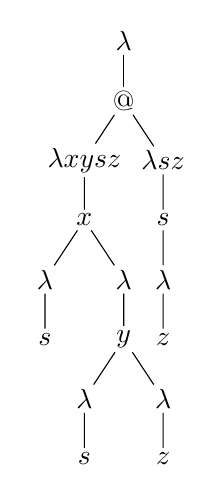
\begin{tikzpicture}[baseline=(root.base),level distance=5ex,inner ysep=0.5mm,sibling distance=10mm]
\node (root)
{$\lambda$}
child {node{$@$}
    child{node{$\lambda x y s z$}
        child { node{$x$}
            child{node{$\lambda$}{
                child {node {$s$}}}
            }
            child{node{$\lambda$}
                child{node{$y$}
                    child{node{$\lambda$}
                        child{ node {$s$}}
                    }
                    child{node{$\lambda$}
                        child{node{$z$}}}
                }
            }
        }
    }
    child{node{$\lambda s z$}
        child{node{$s$}
            child{node{$\lambda$} child{node{$z$}}}
        }
    }
}
;
\end{tikzpicture}

\begin{itemize}
\item Applying as many deterministic rules as possible gives the following traversal at which point the Opponent must make a choice:

$t_\epsilon = \Pstr[0.7cm]{(n0){\lambda }\ (n1){@}\ (n2-n1){\lambda x y s z}\ (n3-n2){x}\ (n4-n1){\lambda s z}\ (n5-n4){s}\ (n6-n3){\lambda }\ (n7-n2){s}\ (n8-n1){\ghostlmd^3}\ (n9-n0){\ghostvar^2} }$

(For readability we indicate the link label in exponent of the source node when representing traversals.)
The core of $t_\epsilon$ is
$\core{t_\epsilon} = \Pstr[0.7cm]{(n0){\lambda } \cdot (n9-n0){{\ghostvar^2}} }$
and therefore $\pview{\core{t_\epsilon}} =  \lambda \cdot \ghostvar^2$ is a path in  $\betanf{M}$.
This means that $\betanf{M}$ must be of the form $\lambda y s \ldots \cdot y N_1 \ldots \ldots N_q$ for some fresh variable $y$ and $s$ and $q\geq0$.

\item In order to determine what each argument $N_k$ is in the final normal form, we eta-expand by applying rule $\rulename{IVar}$ for each possible argument index $k\geq 1$ and then continue applying the traversal rules.

For $k=1$ we get the traversal:

$t_1 = \Pstr[0.7cm]{(n0){\lambda }\ (n1){@}\ (n2-n1){\lambda x y s z}\ (n3-n2){x}\ (n4-n1){\lambda s z}\
(n5-n4){s}\ (n6-n3){\lambda }\
(n7-n2){s}\ (n8-n1){\ghostlmd^3}\
(n9-n0){\ghostvar^2}
(n10-n9){\ghostlmd^1}
(n11-n8){\ghostvar^1}
(n12-n7){\ghostlmd^1}
(n13-n6){\ghostvar^1}
(n14-n5){\lambda^1}
(n15-n4)z
(n16-n3){\lambda^2}
(n17-n2)y
(n18-n1){\ghostlmd^2}
(n19-n0){\ghostvar^1}
}$

The P-view of the traversal core is
$\pview{\core{t_1}} = \Pstr[0.7cm]{(l){\lambda } \cdot (x-l){\ghostvar^2} \cdot (l1-x){\ghostlmd^1}
\cdot (x2-l){\ghostvar^1}
}$
which means that the normal form is of the form $\lambda y s \ldots \cdot s (y R_1 \ldots R_{q_2}) N_2 \ldots N_q$ for some terms $R_1$, \ldots $R_{q_2}$, and $q,q_2\geq 0$.

\item What should be the value of $q$? In other words, how many more $k$ do we need to look at?  The answer: we need to keep iterating on $k$ until the point where applying the traversal rules will only produce ghost variables and ghost lambda-nodes! Because there is a finite number of nodes in the computation tree, the variable node arities are bounded. Therefore for high enough index $k$, the eta-expansion case from rule \rulenamet{Var} will never be met:
        after applying rule \rulenamet{IVar} on $t_\epsilon$, all subsequent extensions of the traversal will be constructed using repeated applications of rule $\rulename{Lam^\ghostvar}$ or the eta-expanded case of rule $\rulename{Var}$.
     The upper-bound $q$ for $k$ is precisely given by the \emph{arity threshold} of the traversal $t_\epsilon$ as defined in \ref{dfn:arity-threshold}.
     Here we have
     \begin{align*}
     \arth(t_\epsilon)
     = \max \{ & |s^2| , \\
               & |s^1| + (|s^2| - |\lambda|) , \\
               & |x| +  (|s^1| - |\lambda s z|) + (|s^2| - |\lambda|)
               %& |@| + (|x|- |\lambda x y s z |) + (|s^1| - |\lambda s z|) + (|s^2| -|\lambda|) \
               \} \\
    = \max \{   & 0 , \\
                & 1 + (0 - 0) , \\
                & 2 + (1 - 2) + (0 - 0)
                %& 2 + (2 - 4) + (1 - 2) + (0 - 0)
            \} \\
     = 1
     \end{align*}
     Thus we don't need to look at higher value of $k$ at $t_\epsilon$, we thus have:
     $\betanf{M} = \lambda y s \ldots \cdot s (y R_1 \ldots R_{q_2})$.

\item The arity threshold of $t_1$ is $\arth(t_1) = |z| + |y| - |\lambda^2| = 0+2-0 = 2$ hence  $\betanf{M}$ is of the form $\lambda y s \ldots \cdot s (y R_1 R_2)$.

\item Let's eta-expand using rule \rulenamet{IVar} for varying value of child index $1\leq k_2 \leq q_2 = 2$. We first look at the case $k_2 = 1$. The traversal obtained is:

$t_{11} = \Pstr[0.7cm]{
(n0){\lambda }\
(n1){@}\ (n2-n1){\lambda x y s z}\ (n3-n2){x}\ (n4-n1){\lambda s z}\ (n5-n4){s}\ (n6-n3){\lambda }\ (n7-n2){s}\ (n8-n1){\ghostlmd^3}\ (n9-n0){\ghostvar^2}
(n10-n9){\ghostlmd^1}
(n11-n8){\ghostvar^1}
(n12-n7){\ghostlmd^1}
(n13-n6){\ghostvar^1}
(n14-n5){\lambda^1}
(n15-n4)z
(n16-n3){\lambda^2}
(n17-n2)y
(n18-n1){\ghostlmd^2}
(n19-n0){\ghostvar^1}
(n20-n19){\ghostlmd^1}
(n21-n18){\ghostvar^1}
(n22-n17,60:1)\lambda % points to non-ghost node
(n23-n2,45:3) s
(n24-n1,45:3) {\ghostlmd^3}
(n25-n0,48:2) {\ghostvar^2}
}$

Thus $\pview{\core{t_{11}}} =
\Pstr[0.7cm]{
(n0){\lambda }\
 (n9-n0){\ghostvar^2}
 (n10-n9){\ghostlmd^1}
(n19-n0){\ghostvar^1}
(n20-n19){\ghostlmd^1}
(n25-n0,48:2){\ghostvar^2}
}$

Hence $\betanf{M}$ is of the form $\lambda y s \ldots \cdot s\ (y\ s\ R_2)$.

\item Now let's extend $t_1$ with \rulenamet{IVar^\lambda} for $k_2 = 2$. We get the traversal:

$t_{12} = \Pstr[0.7cm]{
(n0){\lambda }\
(n1){@}\ (n2-n1){\lambda x y s z}\
(n3-n2){x}\ (n4-n1){\lambda s z}\
(n5-n4){s}\
(n6-n3){\lambda }\
(n7-n2){s}\
(n8-n1){\ghostlmd^3}\
(n9-n0) {\ghostvar^2}
(n10-n9) {\ghostlmd^1}
(n11-n8){\ghostvar^1}
(n12-n7){\ghostlmd^1}
(n13-n6){\ghostvar^1}
(n14-n5)\lambda^1
(n15-n4)z
(n16-n3){\lambda^2}
(n17-n2)y
(n18-n1){\ghostlmd^2}
(n19-n0){\ghostvar^1}
(n20-n19){\ghostlmd^2} %%%%%%%%
(n21-n18){\ghostvar^2}
(n22-n17,60:2)\lambda % points to non-ghost node
(n23-n2,45:4) z
(n24-n1,45:4) {\ghostlmd^4}
(n25-n0,48:3) {\ghostvar^3}
}$

Thus $\pview{\core{t_{12}}} =
\Pstr[0.7cm]{
(n0){\lambda }\
 (n9-n0){{\ghostvar^2}}
 (n10-n9){\ghostlmd^1}
(n19-n0){\ghostvar^1}
(n20-n19){\ghostlmd^2}
(n25-n0,48:3) {\ghostvar^3}
}$

Hence $\betanf{M} = \lambda y s z \cdot s\ (y\ s\ z)$.
\end{itemize}
\end{example}

\begin{example}[``Missing operand'' example by Neil Jones]
\label{ex:missingoperand}
This small example illustrates how on-the-fly eta-expansion helps resolve the ``missing argument'' problem faced when using the traversal rules of STLC. Take $M = (\lambda u . u\ (y_1\ u)) (\lambda v . v\ y_2)$.

The computation tree is:
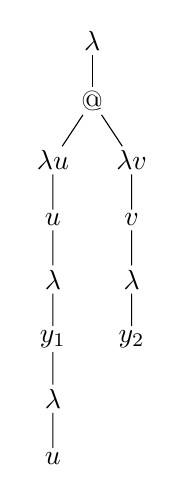
\begin{tikzpicture}[baseline=(root.base),level distance=5ex,inner ysep=0.5mm,sibling distance=10mm]
\node (root)
{$\lambda$}
child {node{$@$}
        child{node{$\lambda u $}
           child {node {$u$}
              child {node {$\lambda$}
                  child {node {$y_1$}
                      child {node {$\lambda$}
                          child {node {$u$}
                          }
                      }
                  }
              }
           }
        }
        child{node{$\lambda v$}
            child{node{$v$}
                child{node{$\lambda$}
                    child{ node {$y_2$}}
                }
            }
        }
    }
;
\end{tikzpicture}

The only two maximal normalizing traversals are:
\begin{itemize}

\item $t_1 = \Pstr[0.7cm]{(n0){\lambda }\ (n1){@}\ (n2-n1){\lambda u}\ (n3-n2){u}\ (n4-n1){\lambda v}\ (n5-n4){v}\ (n6-n3){\lambda }\ (n7-n0){y_1}\ (n8-n7){\lambda }\ (n9-n2){u}\ (n10-n1){\lambda v}\ (n11-n10){v}\ (n12-n9){{\ghostlmd^{1}}}\ (n13-n8){{\ghostvar^{1}}}\ (n14-n13){{\ghostlmd^{1}}}\ (n15-n12){{\ghostvar^{1}}}\ (n16-n11){\lambda }\ (n17-n0,35){y_2}\ }$
\item $t_2 = \Pstr[0.7cm]{(n0){\lambda }\ (n1){@}\ (n2-n1){\lambda u}\ (n3-n2){u}\ (n4-n1){\lambda v}\ (n5-n4){v}\ (n6-n3){\lambda }\ (n7-n0){y_1}\ (n8-n7){{\ghostlmd^{2}}}\ (n9-n6){{\ghostvar^{1}}}\ (n10-n5){\lambda }\ (n11-n0){y_2}\ }$
\end{itemize}
Using the STLC traversals, one can traverse $t_1$ all the way to variable $v$ at which point one get stuck due to the lack of operand applied to the last occurrence of $u$ (the occurrence  at the bottom of the left branch in the tree). Using ULC rule, that operands gets created on-the-fly through eta-expansion and is represented by ghost lambda node $\ghostlmd^1$.

The two core P-views give the two maximal paths in the beta-normal form of $M$:
\begin{itemize}
\item $\pview{\core{t_1}} = \Pstr[0.7cm]{(n0){\lambda }\ (n1-n0){y_1}\ (n2-n1){\lambda }\ (n3-n2){{\ghostvar^{1}}}\ (n4-n3){{\ghostlmd^{1}}}\ (n5-n0){y2}\ }$
\item $\pview{\core{t_2}} = \Pstr[0.7cm]{(n0){\lambda }\ (n1-n0){y_1}\ (n2-n1){{\ghostlmd^{2}}}\ (n3-n0){y_2}\ }$
\end{itemize}
Thus: $\betanf{M} = \lambda x . y_1 (\lambda  z.z\ y_2) y_2$.
\end{example}


\begin{example}[Neil Jones' ``$varity\ 2$'' example]

Take $M = varity\ two$ where
\begin{align*}
  varity &\equiv \lambda t.t (\lambda n a x . n (\lambda s z . a s (x s z))) (\lambda a. a) (\lambda z_0 . z_0) \\
  two &\equiv \lambda s_2 z_2 . s_2 (s_2\ z_2)
\end{align*}

In order to compute the set of normalizing traversals, we apply the traversal rules inductively until an input variable is reached, at which point we eta-expand with rule \rulenamet{IVar} for all possible values of $k$ ranging from $1$ to the arity threshold of the traversal. The first traversal obtained is denoted $t_\epsilon$, and for every sequence of integer $s \in \nat^*$,  the traversal $t_{s \cdot k}$ represents the maximal traversal obtained after extending $t_s$ using one application of the eta-expanded subcase of rule \rulenamet{IVar} with link-label $k \in \nat$.
This process yields the set of traversals $\{t_\epsilon, t_{11}, t_{12}, t_{121}, t_{122} \}$. Table \ref{tab:varity2_trav_epsilon} represents $t_\epsilon$ and
Table \ref{tab:varity2_trav} represents the three maximal traversals $t_{11}, t_{121}, t_{122}$.

\begin{table}
\label{tab:varity2_trav_epsilon}
\resizebox{1.1\hsize}{!}{$
t_\epsilon = \Pstr[0.7cm]{(n0){\lambda }\ (n1){@}\ (n2-n1){\lambda t}\ (n3-n2){t}\ (n4-n1){\lambda s_2 z_2}\ (n5-n4){s_2}\ (n6-n3){\lambda n a x}\ (n7-n6){n}\ (n8-n5){\lambda }\ (n9-n4){s_2}\ (n10-n3){\lambda n a x}\ (n11-n10){n}\ (n12-n9){\lambda }\ (n13-n4){z_2}\ (n14-n3){\lambda a}\ (n15-n14){a}\ (n16-n13){{\ghostlmd^{1}}}\ (n17-n12){{\ghostvar^{1}}}\ (n18-n11){\lambda s z}\ (n19-n10){a}\ (n20-n9){{\ghostlmd^{2}}}\ (n21-n8){{\ghostvar^{1}}}\ (n22-n7){\lambda s z}\ (n23-n6){a}\ (n24-n5){{\ghostlmd^{2}}}\ (n25-n4){{\ghostvar^{3}}}\
(n26-n3){\lambda z_0}\ (n27-n26){z_0}\ (n28-n25){{\ghostlmd^{1}}}\ (n29-n24){{\ghostvar^{1}}}\
(n30-n23){\lambda }\ (n31-n22){s}\ (n32-n21){{\ghostlmd^{1}}}\ (n33-n20){{\ghostvar^{1}}}\ (n34-n19){\lambda }\ (n35-n18){s}\ (n36-n17){{\ghostlmd^{1}}}\ (n37-n16){{\ghostvar^{1}}}\ (n38-n15){{\ghostlmd^{1}}}\ (n39-n14){{\ghostvar^{2}}}\ (n40-n13){{\ghostlmd^{2}}}\ (n41-n12){{\ghostvar^{2}}}\ (n42-n11){{\ghostlmd^{2}}}\ (n43-n10){{\ghostvar^{4}}}\ (n44-n9){{\ghostlmd^{4}}}\ (n45-n8){{\ghostvar^{3}}}\ (n46-n7){{\ghostlmd^{3}}}\ (n47-n6){{\ghostvar^{5}}}\ (n48-n5){{\ghostlmd^{5}}}\ (n49-n4){{\ghostvar^{6}}}\ (n50-n3){{\ghostlmd^{6}}}\ (n51-n2){{\ghostvar^{4}}}\ (n52-n1){{\ghostlmd^{4}}}\ (n53-n0){{\ghostvar^{3}}}}$}
\caption{Traversal $t_\epsilon$ of $varity\ 2$}
\end{table}

\newgeometry{left=1cm,right=2cm, bottom=2cm, top=2cm}
\begin{landscape}
\thispagestyle{empty}
\begin{table}
\label{tab:varity2_trav}
% \resizebox{1.1\hsize}{!}{$t_{1} = \Pstr[0.7cm]{(n0){\lambda }\ (n1){@}\ (n2-n1){\lambda t}\ (n3-n2){t}\ (n4-n1){\lambda s_2 z_2}\ (n5-n4){s_2}\ (n6-n3){\lambda n a x}\ (n7-n6){n}\ (n8-n5){\lambda }\ (n9-n4){s_2}\ (n10-n3){\lambda n a x}\ (n11-n10){n}\ (n12-n9){\lambda }\ (n13-n4){z_2}\ (n14-n3){\lambda a}\ (n15-n14){a}\ (n16-n13){{\ghostlmd^{1}}}\ (n17-n12){{\ghostvar^{1}}}\ (n18-n11){\lambda s z}\ (n19-n10){a}\ (n20-n9){{\ghostlmd^{2}}}\ (n21-n8){{\ghostvar^{1}}}\ (n22-n7){\lambda s z}\ (n23-n6){a}\ (n24-n5){{\ghostlmd^{2}}}\ (n25-n4){{\ghostvar^{3}}}\ (n26-n3){\lambda z_0}\ (n27-n26){z_0}\ (n28-n25){{\ghostlmd^{1}}}\ (n29-n24){{\ghostvar^{1}}}\ (n30-n23){\lambda }\ (n31-n22){s}\ (n32-n21){{\ghostlmd^{1}}}\ (n33-n20){{\ghostvar^{1}}}\ (n34-n19){\lambda }\ (n35-n18){s}\ (n36-n17){{\ghostlmd^{1}}}\ (n37-n16){{\ghostvar^{1}}}\ (n38-n15){{\ghostlmd^{1}}}\ (n39-n14){{\ghostvar^{2}}}\ (n40-n13){{\ghostlmd^{2}}}\ (n41-n12){{\ghostvar^{2}}}\ (n42-n11){{\ghostlmd^{2}}}\ (n43-n10){{\ghostvar^{4}}}\ (n44-n9){{\ghostlmd^{4}}}\ (n45-n8){{\ghostvar^{3}}}\ (n46-n7){{\ghostlmd^{3}}}\ (n47-n6){{\ghostvar^{5}}}\ (n48-n5){{\ghostlmd^{5}}}\ (n49-n4){{\ghostvar^{6}}}\ (n50-n3){{\ghostlmd^{6}}}\ (n51-n2){{\ghostvar^{4}}}\ (n52-n1){{\ghostlmd^{4}}}\ (n53-n0){{\ghostvar^{3}}}\ (n54-n53){{\ghostlmd^{1}}}\ (n55-n52){{\ghostvar^{1}}}\ (n56-n51){{\ghostlmd^{1}}}\ (n57-n50){{\ghostvar^{1}}}\ (n58-n49){{\ghostlmd^{1}}}\ (n59-n48){{\ghostvar^{1}}}\ (n60-n47){{\ghostlmd^{1}}}\ (n61-n46){{\ghostvar^{1}}}\ (n62-n45){{\ghostlmd^{1}}}\ (n63-n44){{\ghostvar^{1}}}\ (n64-n43){{\ghostlmd^{1}}}\ (n65-n42){{\ghostvar^{1}}}\ (n66-n41){{\ghostlmd^{1}}}\ (n67-n40){{\ghostvar^{1}}}\ (n68-n39){{\ghostlmd^{1}}}\ (n69-n38){{\ghostvar^{1}}}\ (n70-n37){{\ghostlmd^{1}}}\ (n71-n36){{\ghostvar^{1}}}\ (n72-n35){{\ghostlmd^{1}}}\ (n73-n34){{\ghostvar^{1}}}\ (n74-n33){{\ghostlmd^{1}}}\ (n75-n32){{\ghostvar^{1}}}\ (n76-n31){{\ghostlmd^{1}}}\ (n77-n30){{\ghostvar^{1}}}\ (n78-n29){{\ghostlmd^{1}}}\ (n79-n28){{\ghostvar^{1}}}\ (n80-n27){{\ghostlmd^{1}}}\ (n81-n26){{\ghostvar^{2}}}\ (n82-n25){{\ghostlmd^{2}}}\ (n83-n24){{\ghostvar^{2}}}\ (n84-n23){\lambda }\ (n85-n6){x}\ (n86-n5){{\ghostlmd^{3}}}\ (n87-n4){{\ghostvar^{4}}}\ (n88-n3){{\ghostlmd^{4}}}\ (n89-n2){{\ghostvar^{2}}}\ (n90-n1){{\ghostlmd^{2}}}\ (n91-n0){{\ghostvar^{1}}}}$}
\resizebox{1\hsize}{!}{$t_{11} = \Pstr[0.7cm]{(n0){\lambda }\ (n1){@}\ (n2-n1){\lambda t}\ (n3-n2){t}\ (n4-n1){\lambda s_2 z_2}\ (n5-n4){s_2}\ (n6-n3){\lambda n a x}\ (n7-n6){n}\ (n8-n5){\lambda }\ (n9-n4){s_2}\ (n10-n3){\lambda n a x}\ (n11-n10){n}\ (n12-n9){\lambda }\ (n13-n4){z_2}\ (n14-n3){\lambda a}\ (n15-n14){a}\ (n16-n13){{\ghostlmd^{1}}}\ (n17-n12){{\ghostvar^{1}}}\ (n18-n11){\lambda s z}\ (n19-n10){a}\ (n20-n9){{\ghostlmd^{2}}}\ (n21-n8){{\ghostvar^{1}}}\ (n22-n7){\lambda s z}\ (n23-n6){a}\ (n24-n5){{\ghostlmd^{2}}}\ (n25-n4){{\ghostvar^{3}}}\ (n26-n3){\lambda z_0}\ (n27-n26){z_0}\ (n28-n25){{\ghostlmd^{1}}}\ (n29-n24){{\ghostvar^{1}}}\ (n30-n23){\lambda }\ (n31-n22){s}\ (n32-n21){{\ghostlmd^{1}}}\ (n33-n20){{\ghostvar^{1}}}\ (n34-n19){\lambda }\ (n35-n18){s}\ (n36-n17){{\ghostlmd^{1}}}\ (n37-n16){{\ghostvar^{1}}}\ (n38-n15){{\ghostlmd^{1}}}\ (n39-n14){{\ghostvar^{2}}}\ (n40-n13){{\ghostlmd^{2}}}\ (n41-n12){{\ghostvar^{2}}}\ (n42-n11){{\ghostlmd^{2}}}\ (n43-n10){{\ghostvar^{4}}}\ (n44-n9){{\ghostlmd^{4}}}\ (n45-n8){{\ghostvar^{3}}}\ (n46-n7){{\ghostlmd^{3}}}\ (n47-n6){{\ghostvar^{5}}}\ (n48-n5){{\ghostlmd^{5}}}\ (n49-n4){{\ghostvar^{6}}}\ (n50-n3){{\ghostlmd^{6}}}\ (n51-n2){{\ghostvar^{4}}}\ (n52-n1){{\ghostlmd^{4}}}\ (n53-n0){{\ghostvar^{3}}}\ (n54-n53){{\ghostlmd^{1}}}\ (n55-n52){{\ghostvar^{1}}}\ (n56-n51){{\ghostlmd^{1}}}\ (n57-n50){{\ghostvar^{1}}}\ (n58-n49){{\ghostlmd^{1}}}\ (n59-n48){{\ghostvar^{1}}}\ (n60-n47){{\ghostlmd^{1}}}\ (n61-n46){{\ghostvar^{1}}}\ (n62-n45){{\ghostlmd^{1}}}\ (n63-n44){{\ghostvar^{1}}}\ (n64-n43){{\ghostlmd^{1}}}\ (n65-n42){{\ghostvar^{1}}}\ (n66-n41){{\ghostlmd^{1}}}\ (n67-n40){{\ghostvar^{1}}}\ (n68-n39){{\ghostlmd^{1}}}\ (n69-n38){{\ghostvar^{1}}}\ (n70-n37){{\ghostlmd^{1}}}\ (n71-n36){{\ghostvar^{1}}}\ (n72-n35){{\ghostlmd^{1}}}\ (n73-n34){{\ghostvar^{1}}}\ (n74-n33){{\ghostlmd^{1}}}\ (n75-n32){{\ghostvar^{1}}}\ (n76-n31){{\ghostlmd^{1}}}\ (n77-n30){{\ghostvar^{1}}}\ (n78-n29){{\ghostlmd^{1}}}\ (n79-n28){{\ghostvar^{1}}}\ (n80-n27){{\ghostlmd^{1}}}\ (n81-n26){{\ghostvar^{2}}}\ (n82-n25){{\ghostlmd^{2}}}\ (n83-n24){{\ghostvar^{2}}}\ (n84-n23){\lambda }\ (n85-n6){x}\ (n86-n5){{\ghostlmd^{3}}}\ (n87-n4){{\ghostvar^{4}}}\ (n88-n3){{\ghostlmd^{4}}}\ (n89-n2){{\ghostvar^{2}}}\ (n90-n1){{\ghostlmd^{2}}}\ (n91-n0){{\ghostvar^{1}}}\ (n92-n91){{\ghostlmd^{1}}}\ (n93-n90){{\ghostvar^{1}}}\ (n94-n89){{\ghostlmd^{1}}}\ (n95-n88){{\ghostvar^{1}}}\ (n96-n87){{\ghostlmd^{1}}}\ (n97-n86){{\ghostvar^{1}}}\ (n98-n85){\lambda }\ (n99-n22){s}\ (n100-n21){{\ghostlmd^{1}}}\ (n101-n20){{\ghostvar^{1}}}\ (n102-n19){\lambda }\ (n103-n18){s}\ (n104-n17){{\ghostlmd^{1}}}\ (n105-n16){{\ghostvar^{1}}}\ (n106-n15){{\ghostlmd^{1}}}\ (n107-n14){{\ghostvar^{2}}}\ (n108-n13){{\ghostlmd^{2}}}\ (n109-n12){{\ghostvar^{2}}}\ (n110-n11){{\ghostlmd^{2}}}\ (n111-n10){{\ghostvar^{4}}}\ (n112-n9){{\ghostlmd^{4}}}\ (n113-n8){{\ghostvar^{3}}}\ (n114-n7){{\ghostlmd^{3}}}\ (n115-n6){{\ghostvar^{5}}}\ (n116-n5){{\ghostlmd^{5}}}\ (n117-n4){{\ghostvar^{6}}}\ (n118-n3){{\ghostlmd^{6}}}\ (n119-n2){{\ghostvar^{4}}}\ (n120-n1){{\ghostlmd^{4}}}\ (n121-n0){{\ghostvar^{3}}}}$}
% \resizebox{1.1\hsize}{!}{$t_{12} = \Pstr[0.7cm]{(n0){\lambda }\ (n1){@}\ (n2-n1){\lambda t}\ (n3-n2){t}\ (n4-n1){\lambda s_2 z_2}\ (n5-n4){s_2}\ (n6-n3){\lambda n a x}\ (n7-n6){n}\ (n8-n5){\lambda }\ (n9-n4){s_2}\ (n10-n3){\lambda n a x}\ (n11-n10){n}\ (n12-n9){\lambda }\ (n13-n4){z_2}\ (n14-n3){\lambda a}\ (n15-n14){a}\ (n16-n13){{\ghostlmd^{1}}}\ (n17-n12){{\ghostvar^{1}}}\ (n18-n11){\lambda s z}\ (n19-n10){a}\ (n20-n9){{\ghostlmd^{2}}}\ (n21-n8){{\ghostvar^{1}}}\ (n22-n7){\lambda s z}\ (n23-n6){a}\ (n24-n5){{\ghostlmd^{2}}}\ (n25-n4){{\ghostvar^{3}}}\ (n26-n3){\lambda z_0}\ (n27-n26){z_0}\ (n28-n25){{\ghostlmd^{1}}}\ (n29-n24){{\ghostvar^{1}}}\ (n30-n23){\lambda }\ (n31-n22){s}\ (n32-n21){{\ghostlmd^{1}}}\ (n33-n20){{\ghostvar^{1}}}\ (n34-n19){\lambda }\ (n35-n18){s}\ (n36-n17){{\ghostlmd^{1}}}\ (n37-n16){{\ghostvar^{1}}}\ (n38-n15){{\ghostlmd^{1}}}\ (n39-n14){{\ghostvar^{2}}}\ (n40-n13){{\ghostlmd^{2}}}\ (n41-n12){{\ghostvar^{2}}}\ (n42-n11){{\ghostlmd^{2}}}\ (n43-n10){{\ghostvar^{4}}}\ (n44-n9){{\ghostlmd^{4}}}\ (n45-n8){{\ghostvar^{3}}}\ (n46-n7){{\ghostlmd^{3}}}\ (n47-n6){{\ghostvar^{5}}}\ (n48-n5){{\ghostlmd^{5}}}\ (n49-n4){{\ghostvar^{6}}}\ (n50-n3){{\ghostlmd^{6}}}\ (n51-n2){{\ghostvar^{4}}}\ (n52-n1){{\ghostlmd^{4}}}\ (n53-n0){{\ghostvar^{3}}}\ (n54-n53){{\ghostlmd^{1}}}\ (n55-n52){{\ghostvar^{1}}}\ (n56-n51){{\ghostlmd^{1}}}\ (n57-n50){{\ghostvar^{1}}}\ (n58-n49){{\ghostlmd^{1}}}\ (n59-n48){{\ghostvar^{1}}}\ (n60-n47){{\ghostlmd^{1}}}\ (n61-n46){{\ghostvar^{1}}}\ (n62-n45){{\ghostlmd^{1}}}\ (n63-n44){{\ghostvar^{1}}}\ (n64-n43){{\ghostlmd^{1}}}\ (n65-n42){{\ghostvar^{1}}}\ (n66-n41){{\ghostlmd^{1}}}\ (n67-n40){{\ghostvar^{1}}}\ (n68-n39){{\ghostlmd^{1}}}\ (n69-n38){{\ghostvar^{1}}}\ (n70-n37){{\ghostlmd^{1}}}\ (n71-n36){{\ghostvar^{1}}}\ (n72-n35){{\ghostlmd^{1}}}\ (n73-n34){{\ghostvar^{1}}}\ (n74-n33){{\ghostlmd^{1}}}\ (n75-n32){{\ghostvar^{1}}}\ (n76-n31){{\ghostlmd^{1}}}\ (n77-n30){{\ghostvar^{1}}}\ (n78-n29){{\ghostlmd^{1}}}\ (n79-n28){{\ghostvar^{1}}}\ (n80-n27){{\ghostlmd^{1}}}\ (n81-n26){{\ghostvar^{2}}}\ (n82-n25){{\ghostlmd^{2}}}\ (n83-n24){{\ghostvar^{2}}}\ (n84-n23){\lambda }\ (n85-n6){x}\ (n86-n5){{\ghostlmd^{3}}}\ (n87-n4){{\ghostvar^{4}}}\ (n88-n3){{\ghostlmd^{4}}}\ (n89-n2){{\ghostvar^{2}}}\ (n90-n1){{\ghostlmd^{2}}}\ (n91-n0){{\ghostvar^{1}}}\ (n92-n91){{\ghostlmd^{2}}}\ (n93-n90){{\ghostvar^{2}}}\ (n94-n89){{\ghostlmd^{2}}}\ (n95-n88){{\ghostvar^{2}}}\ (n96-n87){{\ghostlmd^{2}}}\ (n97-n86){{\ghostvar^{2}}}\ (n98-n85){\lambda }\ (n99-n22){z}\ (n100-n21){{\ghostlmd^{2}}}\ (n101-n20){{\ghostvar^{2}}}\ (n102-n19){\lambda }\ (n103-n10){x}\ (n104-n9){{\ghostlmd^{3}}}\ (n105-n8){{\ghostvar^{2}}}\ (n106-n7){{\ghostlmd^{2}}}\ (n107-n6){{\ghostvar^{4}}}\ (n108-n5){{\ghostlmd^{4}}}\ (n109-n4){{\ghostvar^{5}}}\ (n110-n3){{\ghostlmd^{5}}}\ (n111-n2){{\ghostvar^{3}}}\ (n112-n1){{\ghostlmd^{3}}}\ (n113-n0){{\ghostvar^{2}}}}$}
\resizebox{1\hsize}{!}{$t_{121} =
\Pstr[0.7cm]{(n0){\lambda }\ (n1){@}\ (n2-n1){\lambda t}\ (n3-n2){t}\ (n4-n1){\lambda s_2 z_2}\ (n5-n4){s_2}\ (n6-n3){\lambda n a x}\ (n7-n6){n}\ (n8-n5){\lambda }\ (n9-n4){s_2}\ (n10-n3){\lambda n a x}\ (n11-n10){n}\ (n12-n9){\lambda }\ (n13-n4){z_2}\ (n14-n3){\lambda a}\ (n15-n14){a}\ (n16-n13){{\ghostlmd^{1}}}\ (n17-n12){{\ghostvar^{1}}}\ (n18-n11){\lambda s z}\ (n19-n10){a}\ (n20-n9){{\ghostlmd^{2}}}\ (n21-n8){{\ghostvar^{1}}}\ (n22-n7){\lambda s z}\ (n23-n6){a}\ (n24-n5){{\ghostlmd^{2}}}\ (n25-n4){{\ghostvar^{3}}}\ (n26-n3){\lambda z_0}\ (n27-n26){z_0}\ (n28-n25){{\ghostlmd^{1}}}\ (n29-n24){{\ghostvar^{1}}}\ (n30-n23){\lambda }\ (n31-n22){s}\ (n32-n21){{\ghostlmd^{1}}}\ (n33-n20){{\ghostvar^{1}}}\ (n34-n19){\lambda }\ (n35-n18){s}\ (n36-n17){{\ghostlmd^{1}}}\ (n37-n16){{\ghostvar^{1}}}\ (n38-n15){{\ghostlmd^{1}}}\ (n39-n14){{\ghostvar^{2}}}\ (n40-n13){{\ghostlmd^{2}}}\ (n41-n12){{\ghostvar^{2}}}\ (n42-n11){{\ghostlmd^{2}}}\ (n43-n10){{\ghostvar^{4}}}\ (n44-n9){{\ghostlmd^{4}}}\ (n45-n8){{\ghostvar^{3}}}\ (n46-n7){{\ghostlmd^{3}}}\ (n47-n6){{\ghostvar^{5}}}\ (n48-n5){{\ghostlmd^{5}}}\ (n49-n4){{\ghostvar^{6}}}\ (n50-n3){{\ghostlmd^{6}}}\ (n51-n2){{\ghostvar^{4}}}\ (n52-n1){{\ghostlmd^{4}}}\ (n53-n0){{\ghostvar^{3}}}\ (n54-n53){{\ghostlmd^{1}}}\ (n55-n52){{\ghostvar^{1}}}\ (n56-n51){{\ghostlmd^{1}}}\ (n57-n50){{\ghostvar^{1}}}\ (n58-n49){{\ghostlmd^{1}}}\ (n59-n48){{\ghostvar^{1}}}\ (n60-n47){{\ghostlmd^{1}}}\ (n61-n46){{\ghostvar^{1}}}\ (n62-n45){{\ghostlmd^{1}}}\ (n63-n44){{\ghostvar^{1}}}\ (n64-n43){{\ghostlmd^{1}}}\ (n65-n42){{\ghostvar^{1}}}\ (n66-n41){{\ghostlmd^{1}}}\ (n67-n40){{\ghostvar^{1}}}\ (n68-n39){{\ghostlmd^{1}}}\ (n69-n38){{\ghostvar^{1}}}\ (n70-n37){{\ghostlmd^{1}}}\ (n71-n36){{\ghostvar^{1}}}\ (n72-n35){{\ghostlmd^{1}}}\ (n73-n34){{\ghostvar^{1}}}\ (n74-n33){{\ghostlmd^{1}}}\ (n75-n32){{\ghostvar^{1}}}\ (n76-n31){{\ghostlmd^{1}}}\ (n77-n30){{\ghostvar^{1}}}\ (n78-n29){{\ghostlmd^{1}}}\ (n79-n28){{\ghostvar^{1}}}\ (n80-n27){{\ghostlmd^{1}}}\ (n81-n26){{\ghostvar^{2}}}\ (n82-n25){{\ghostlmd^{2}}}\ (n83-n24){{\ghostvar^{2}}}\ (n84-n23){\lambda }\ (n85-n6){x}\ (n86-n5){{\ghostlmd^{3}}}\ (n87-n4){{\ghostvar^{4}}}\ (n88-n3){{\ghostlmd^{4}}}\ (n89-n2){{\ghostvar^{2}}}\ (n90-n1){{\ghostlmd^{2}}}\ (n91-n0){{\ghostvar^{1}}}\ (n92-n91){{\ghostlmd^{2}}}\ (n93-n90){{\ghostvar^{2}}}\ (n94-n89){{\ghostlmd^{2}}}\ (n95-n88){{\ghostvar^{2}}}\ (n96-n87){{\ghostlmd^{2}}}\ (n97-n86){{\ghostvar^{2}}}\ (n98-n85){\lambda }\ (n99-n22){z}\ (n100-n21){{\ghostlmd^{2}}}\ (n101-n20){{\ghostvar^{2}}}\ (n102-n19){\lambda }\ (n103-n10){x}\ (n104-n9){{\ghostlmd^{3}}}\ (n105-n8){{\ghostvar^{2}}}\ (n106-n7){{\ghostlmd^{2}}}\ (n107-n6){{\ghostvar^{4}}}\ (n108-n5){{\ghostlmd^{4}}}\ (n109-n4){{\ghostvar^{5}}}\ (n110-n3){{\ghostlmd^{5}}}\ (n111-n2){{\ghostvar^{3}}}\ (n112-n1){{\ghostlmd^{3}}}\ (n113-n0){{\ghostvar^{2}}}\ (n114-n113){{\ghostlmd^{1}}}\ (n115-n112){{\ghostvar^{1}}}\ (n116-n111){{\ghostlmd^{1}}}\ (n117-n110){{\ghostvar^{1}}}\ (n118-n109){{\ghostlmd^{1}}}\ (n119-n108){{\ghostvar^{1}}}\ (n120-n107){{\ghostlmd^{1}}}\ (n121-n106){{\ghostvar^{1}}}\ (n122-n105){{\ghostlmd^{1}}}\ (n123-n104){{\ghostvar^{1}}}\ (n124-n103){\lambda }\ (n125-n18){s}\ (n126-n17){{\ghostlmd^{1}}}\ (n127-n16){{\ghostvar^{1}}}\ (n128-n15){{\ghostlmd^{1}}}\ (n129-n14){{\ghostvar^{2}}}\ (n130-n13){{\ghostlmd^{2}}}\ (n131-n12){{\ghostvar^{2}}}\ (n132-n11){{\ghostlmd^{2}}}\ (n133-n10){{\ghostvar^{4}}}\ (n134-n9){{\ghostlmd^{4}}}\ (n135-n8){{\ghostvar^{3}}}\ (n136-n7){{\ghostlmd^{3}}}\ (n137-n6){{\ghostvar^{5}}}\ (n138-n5){{\ghostlmd^{5}}}\ (n139-n4){{\ghostvar^{6}}}\ (n140-n3){{\ghostlmd^{6}}}\ (n141-n2){{\ghostvar^{4}}}\ (n142-n1){{\ghostlmd^{4}}}\ (n143-n0){{\ghostvar^{3}}}}$}

\resizebox{1\hsize}{!}{$t_{122} =
\Pstr[0.7cm]{(n0){\lambda }\ (n1){@}\ (n2-n1){\lambda t}\ (n3-n2){t}\ (n4-n1){\lambda s_2 z_2}\ (n5-n4){s_2}\ (n6-n3){\lambda n a x}\ (n7-n6){n}\ (n8-n5){\lambda }\ (n9-n4){s_2}\ (n10-n3){\lambda n a x}\ (n11-n10){n}\ (n12-n9){\lambda }\ (n13-n4){z_2}\ (n14-n3){\lambda a}\ (n15-n14){a}\ (n16-n13){{\ghostlmd^{1}}}\ (n17-n12){{\ghostvar^{1}}}\ (n18-n11){\lambda s z}\ (n19-n10){a}\ (n20-n9){{\ghostlmd^{2}}}\ (n21-n8){{\ghostvar^{1}}}\ (n22-n7){\lambda s z}\ (n23-n6){a}\ (n24-n5){{\ghostlmd^{2}}}\ (n25-n4){{\ghostvar^{3}}}\ (n26-n3){\lambda z_0}\ (n27-n26){z_0}\ (n28-n25){{\ghostlmd^{1}}}\ (n29-n24){{\ghostvar^{1}}}\ (n30-n23){\lambda }\ (n31-n22){s}\ (n32-n21){{\ghostlmd^{1}}}\ (n33-n20){{\ghostvar^{1}}}\ (n34-n19){\lambda }\ (n35-n18){s}\ (n36-n17){{\ghostlmd^{1}}}\ (n37-n16){{\ghostvar^{1}}}\ (n38-n15){{\ghostlmd^{1}}}\ (n39-n14){{\ghostvar^{2}}}\ (n40-n13){{\ghostlmd^{2}}}\ (n41-n12){{\ghostvar^{2}}}\ (n42-n11){{\ghostlmd^{2}}}\ (n43-n10){{\ghostvar^{4}}}\ (n44-n9){{\ghostlmd^{4}}}\ (n45-n8){{\ghostvar^{3}}}\ (n46-n7){{\ghostlmd^{3}}}\ (n47-n6){{\ghostvar^{5}}}\ (n48-n5){{\ghostlmd^{5}}}\ (n49-n4){{\ghostvar^{6}}}\ (n50-n3){{\ghostlmd^{6}}}\ (n51-n2){{\ghostvar^{4}}}\ (n52-n1){{\ghostlmd^{4}}}\ (n53-n0){{\ghostvar^{3}}}\ (n54-n53){{\ghostlmd^{1}}}\ (n55-n52){{\ghostvar^{1}}}\ (n56-n51){{\ghostlmd^{1}}}\ (n57-n50){{\ghostvar^{1}}}\ (n58-n49){{\ghostlmd^{1}}}\ (n59-n48){{\ghostvar^{1}}}\ (n60-n47){{\ghostlmd^{1}}}\ (n61-n46){{\ghostvar^{1}}}\ (n62-n45){{\ghostlmd^{1}}}\ (n63-n44){{\ghostvar^{1}}}\ (n64-n43){{\ghostlmd^{1}}}\ (n65-n42){{\ghostvar^{1}}}\ (n66-n41){{\ghostlmd^{1}}}\ (n67-n40){{\ghostvar^{1}}}\ (n68-n39){{\ghostlmd^{1}}}\ (n69-n38){{\ghostvar^{1}}}\ (n70-n37){{\ghostlmd^{1}}}\ (n71-n36){{\ghostvar^{1}}}\ (n72-n35){{\ghostlmd^{1}}}\ (n73-n34){{\ghostvar^{1}}}\ (n74-n33){{\ghostlmd^{1}}}\ (n75-n32){{\ghostvar^{1}}}\ (n76-n31){{\ghostlmd^{1}}}\ (n77-n30){{\ghostvar^{1}}}\ (n78-n29){{\ghostlmd^{1}}}\ (n79-n28){{\ghostvar^{1}}}\ (n80-n27){{\ghostlmd^{1}}}\ (n81-n26){{\ghostvar^{2}}}\ (n82-n25){{\ghostlmd^{2}}}\ (n83-n24){{\ghostvar^{2}}}\ (n84-n23){\lambda }\ (n85-n6){x}\ (n86-n5){{\ghostlmd^{3}}}\ (n87-n4){{\ghostvar^{4}}}\ (n88-n3){{\ghostlmd^{4}}}\ (n89-n2){{\ghostvar^{2}}}\ (n90-n1){{\ghostlmd^{2}}}\ (n91-n0){{\ghostvar^{1}}}\ (n92-n91){{\ghostlmd^{2}}}\ (n93-n90){{\ghostvar^{2}}}\ (n94-n89){{\ghostlmd^{2}}}\ (n95-n88){{\ghostvar^{2}}}\ (n96-n87){{\ghostlmd^{2}}}\ (n97-n86){{\ghostvar^{2}}}\ (n98-n85){\lambda }\ (n99-n22){z}\ (n100-n21){{\ghostlmd^{2}}}\ (n101-n20){{\ghostvar^{2}}}\ (n102-n19){\lambda }\ (n103-n10){x}\ (n104-n9){{\ghostlmd^{3}}}\ (n105-n8){{\ghostvar^{2}}}\ (n106-n7){{\ghostlmd^{2}}}\ (n107-n6){{\ghostvar^{4}}}\ (n108-n5){{\ghostlmd^{4}}}\ (n109-n4){{\ghostvar^{5}}}\ (n110-n3){{\ghostlmd^{5}}}\ (n111-n2){{\ghostvar^{3}}}\ (n112-n1){{\ghostlmd^{3}}}\ (n113-n0){{\ghostvar^{2}}}\ (n114-n113){{\ghostlmd^{2}}}\ (n115-n112){{\ghostvar^{2}}}\ (n116-n111){{\ghostlmd^{2}}}\ (n117-n110){{\ghostvar^{2}}}\ (n118-n109){{\ghostlmd^{2}}}\ (n119-n108){{\ghostvar^{2}}}\ (n120-n107){{\ghostlmd^{2}}}\ (n121-n106){{\ghostvar^{2}}}\ (n122-n105){{\ghostlmd^{2}}}\ (n123-n104){{\ghostvar^{2}}}\ (n124-n103){\lambda }\ (n125-n18){z}\ (n126-n17){{\ghostlmd^{2}}}\ (n127-n16){{\ghostvar^{2}}}\ (n128-n15){{\ghostlmd^{2}}}\ (n129-n14){{\ghostvar^{3}}}\ (n130-n13){{\ghostlmd^{3}}}\ (n131-n12){{\ghostvar^{3}}}\ (n132-n11){{\ghostlmd^{3}}}\ (n133-n10){{\ghostvar^{5}}}\ (n134-n9){{\ghostlmd^{5}}}\ (n135-n8){{\ghostvar^{4}}}\ (n136-n7){{\ghostlmd^{4}}}\ (n137-n6){{\ghostvar^{6}}}\ (n138-n5){{\ghostlmd^{6}}}\ (n139-n4){{\ghostvar^{7}}}\ (n140-n3){{\ghostlmd^{7}}}\ (n141-n2){{\ghostvar^{5}}}\ (n142-n1){{\ghostlmd^{5}}}\ (n143-n0){{\ghostvar^{4}}}}$}
\caption{Maximal traversals of $varity\ 2$}
\end{table}
\end{landscape}
\restoregeometry

Keeping only the maximal traversals gives us the following set of maximal normalizing traversals of $M$:
$$\travsetnorm_{max}(M) = \{ t_{11}, t_{121}, t_{122} \}$$

Hence the set of maximal paths in the beta-normal form of $M$ is given by the traversal core P-views:
\begin{align*}
\pview{\core{t_{11}}} &=
    \Pstr[0.7cm]{(n0){\lambda }\ (n1-n0){{\ghostvar^{3}}}\ (n2-n1){{\ghostlmd^{1}}}\ (n3-n0){{\ghostvar^{1}}}\ (n4-n3){{\ghostlmd^{1}}}\ (n5-n0){{\ghostvar^{3}}}}
\\
\pview{\core{t_{121}}} &=
    \Pstr[0.7cm]{(n0){\lambda }\ (n1-n0){{\ghostvar^{3}}}\ (n2-n1){{\ghostlmd^{1}}}\ (n3-n0){{\ghostvar^{1}}}\ (n4-n3){{\ghostlmd^{2}}}\ (n5-n0){{\ghostvar^{2}}}\ (n6-n5){{\ghostlmd^{1}}}\ (n7-n0){{\ghostvar^{3}}}}
\\
\pview{\core{t_{122}}} &=
\Pstr[0.7cm]{(n0){\lambda }\ (n1-n0){{\ghostvar^{3}}}\ (n2-n1){{\ghostlmd^{1}}}\ (n3-n0){{\ghostvar^{1}}}\ (n4-n3){{\ghostlmd^{2}}}\ (n5-n0){{\ghostvar^{2}}}\ (n6-n5){{\ghostlmd^{2}}}\ (n7-n0){{\ghostvar^{4}}}}
\end{align*}

Therefore the beta-normal from of $varity\ 2$ is:
\begin{align*}
\betanf{varity\ 2} &= \lambda x_1 x_2 x_3 x_4 . x_3 (x_1 x_3 (x_2 x_3 x_4))\\
&\equiv_\alpha \lambda x y s z . s (x s (y s z))
\end{align*}
\end{example}

\section{Further directions}

\subsection{Higher-order collapsible pushdown automata}

In \cite{Ong2006}, a construction\footnote{This CPDA construction from HORS is implemented in the HOG tool.)}
 is defined that converts a higher-order recursion scheme into an equivalent collapsible higher-order pushdown automaton (in the sense that they generate the same infinite tree). The automaton proceeds by calculating traversals over the tree representation of the higher-order recursion scheme. In that setting, the recursion scheme represents a closed term (no free variable) of order-$0$, and the generated structure is an order-$0$ value (a tree).

Conceivably, there must be some kind of tree-generating automaton that can be used to calculate the set of traversals of an untyped lambda term as defined in this paper. The generated tree would be an order-$0$ tree representation of the beta-normal of a term: each terminal symbol of the automaton would correspond to a ``token'' of the lambda term: either a lambda node (represented by non-terminal of type $o->o$), or a variable node (represented by a non-terminal of type $o^k->o$ where $k\geq0$ is the number of operand applied to the variable in the beta normal form of the term.

In the untyped lambda calculus, though, there is no notion of order, therefore the type-based definition of higher-order pushdown automata, where each non-terminals has a simple-type, would not be appropriate here. The definition of HOCPDA would thus need to be relaxed to allow non-terminals of any type. The construction of the HOPCPDA itself would follow the same lines as \cite{Ong2006} except that $\eta$-long normal expansion is not needed.

\subsection{Connection with compilation of ULC to LLL}

In \cite{JonesBerezunLLL}, Daniil Berezun and Neil Jones define a different version of traversals with notable differences: no ghost lambda nodes, two types of justification pointers: binding pointers and control pointers. Although very similar, the relationship between their notion of traversals and the one defined in this paper is still not formally established. Danos and Regnier's Linear Head reduction paper \cite{danos-head} appears to be the best avenue to establish the connection.


\subsection{Game semantics connection}

In the lines of \cite{BlumPhd} where the connection between the theory of traversals and Game Semantics was formalized for typed languages including the simply-typed lambda calculus, PCF and Idealized Algol, a natural question to ask is whether there is a similar connection between the ULC traversals defined in this paper on game models of the untyped lambda calculus. We conjecture that the Game Semantic correspondence can be generalized to the game model of the untyped lambda calculs introduced in Andrew Ker's thesis \cite{KerThesis} in which lambda-terms are denoted by \emph{effectively almost everywhere copycat} strategy  (Conjecture \ref{conj:ulc_corresp}).

\subsection{Head linear reduction}

Traversals have emerged as a constructive method to represent
Relationship between Game Semantics and

In 2004, Danos and Regnier \cite{danos-head} establish the connection between Game Semantics and the notion of \emph{head-linear reduction}.

Head linear reduction is  a non-standard reduction strategy for the lambda calculus and shed some light studies the connection with Game Semantics.


\section{Leftmost linear reduction}
\label{sec:leftmostlinearred}

\subsection{Background: Lambda calculus and reduction}
We recall from standard results of the lambda calculus.
A \defname{redex} is a sub-term of the form $(\lambda x. M) N$.
Reducing redex $(\lambda x. M) N$, or also \emph{firing} the redex, means substituting all free occurrences of $x$ in $M$ by the term $N$ using capture avoiding substitution (the bound variable is renamed afresh when recursively substituting under a lambda).

A term is said to be in \defname{normal form} if it does not contain any redex.
A term is in \defname{head normal form} if it can be written $\lambda x_1 \ldots x_n . y A_1 \ldots A_m$ for $n,m\geq0$. If a term is not in head normal form then its \defname{head beta-redex} is the left-most redex, otherwise the term does not have any head beta-redex.

For any reduction relation $\rightarrow$ between terms we will write
$\rightarrow^*$ to denote its reflexive transitive closure.

The \defname{head reduction}, denoted $\rightarrow_{h}$, fires the head redex of a term if it exists. It can be shown that $\rightarrow^*_{h}$ yields the head-normal form. The \defname{normal-order reduction strategy}, also called leftmost-outermost reduction strategy, performs head reduction until reaching the head-normal form and then recursively applies head reduction on each operand of the head variable. This reduction strategy can be shown to yield the normal form if it exists.


\subsection{Head-linear reduction}
We now introduce the head-linear reduction of Danos-Regnier \cite{danos-head}.

In the standard lambda calculus, a redex is necessarily formed by the outermost lambda in operator position of an application: if the operator consists of consecutive lambda abstractions (\eg, as in $(\lambda x \lambda y . M) A_1 A_2$) then the outermost lambda (\eg, $\lambda x$) is the one that will form the redex. The notion of redex can be generalized to allow evaluation of arguments in any order. In particular, one can allow any of the consecutive $\lambda$-abstractions to form a redex (\eg, the abstraction $\lambda y$ and corresponding argument $A_2$ would be a valid redex). This is formalized by the notion of \emph{generalized redex} (a generalized version of the \emph{prime redex} of Danos-Regnier):

\begin{definition}[Generalized redex]
The set of generalized redexes of a term $M$, written $gr(M)$, is a set of pairs $(\lambda x, A)$ where $\lambda x$ is some abstraction in $M$ and $A$ is a subterm called the argument of $\lambda x$. The head $\lambda$ list of $M$, written $\lambda_l(M)$ is a list of lambda abstractions of $M$. They are defined by induction:
\begin{align*}
gr(v) &= \emptyset & \lambda_l(v) &= \emptyset\\
gr(\lambda x. U) &= gr(U) & \lambda_l(\lambda x. U) &= \lambda x \cdot \lambda_l(U) \\
gr(U V) &= \{ (\lambda x, V) \} \union gr(U) \union gr(V) &
\lambda_l(U V) &= l & \mbox{if $\lambda_l(U) = \lambda x \cdot l$} \\
gr(U V) &= gr(U) \union gr(V) & \lambda_l(U V) &= \epsilon & \mbox{if $\lambda_l(U) = \epsilon$.} \\
\end{align*}
where $v$ ranges over variable occurrences, $x$ ranges over variable names, $U, V$ range over subterms of $M$, and $\epsilon$ denotes the empty list.
\end{definition}

\begin{example} For any term $M, N, A_1, A_2$ we have
(i) $gr((\lambda x \lambda y . M) A_1 A_2) = \{ (\lambda x, A_1), (\lambda y, A_2)\}$ and
(ii) $gr((\lambda z . (\lambda x \lambda y . M) N) A_1 A_2) = \{ (\lambda z, A_1), (\lambda x, N), (\lambda y, A_2)\}$.
\end{example}

Note: In order to define head-linear reduction, one needs to consider specific \emph{occurrences} of variables and sub-terms in a given term. In particular, let's emphasize that when denoting a generalized redex by a pair $(\lambda x, A)$, the component $\lambda x$ and $A$ denote specific \emph{occurrences} of $\lambda x$ and subterm $A$.

We say that a variable occurrence is \defname{involved} in the generalized redex $(\lambda x, A)$ if the variable occurrence is bound by $\lambda x$. A variable occurrence can therefore be involved in at most one generalized redex. We define the \defname{linear substitution} of $x$ for $A$ as the term obtained by performing capture-avoiding substitution of that single occurrence of $x$ by $A$. (Compare this to the standard substitution that applies to \emph{every} occurrence of $x$ in $M$.) When performing such substitution we say that we \defname{linearly fire} the generalized redex $(\lambda x, A)$ for that occurrence of $x$.

We define the \defname{head variable occurrence} of a term as the left-most variable occurring in the term (\ie, the first variable found by depth-first traversal of the term tree.) If the head variable occurrence of a term is involved in a generalized redex then we call that redex the \defname{head-linear redex}.
A term that does not have a head-linear redex is said to be in \defname{quasi head-normal form}.

The \defname{head-linear reduction} $\rightarrow_{hl}$ is defined as the reduction that linearly fires the head linear redex, if it exists. It can be shown that the reflexive transitive closure $\rightarrow^*_{hl}$ yields the quasi head-normal form.

\paragraph{Soundness}
The set of \defname{spine subterms} is defined by induction: a term is a spine subterm of itself; the spine subterms of $U V$ and $\lambda x. U$ are those of $U$.
A \defname{prime redex} (ala Danos-Regner) is a generalized redex $(\lambda x, A)$ such that the operator of the redex ($\lambda x . U$ for some $U$) is a spine subterm.

Danos-Reigner showed the following result:
\begin{theorem}[Soundness and completeness of head-linear reduction \cite{danos-head}]
\label{thm:danosreigner_headlinred}
\begin{compactitem}
\item If $T \rightarrow^*_{hl} T$  then $T$ and $T'$ are $\beta$-equivalent.
\item If $T$ is in quasi-head normal form and has $n$ prime redexes then the head reduction of $T$ leads to a head normal form in exactly $n$ steps.
\item If $T$ is any term, the head linear reduction of $T$ terminates iff the head reduction of $T$ terminates.
\end{compactitem}
\end{theorem}

\subsubsection{Leftmost linear reduction strategy}

As the name indicates, the head-linear reduction is a linear version of the \emph{head} reduction. It thus only yields the quasi \emph{head}-normal form, not the normal form, and therefore is not complete for normalization.

In the standard lambda calculus, normal-order reduction strategy is obtained by repeatedly applying head reduction to get to the head-normal form, and then continuously applying the head-reduction on each argument of the head variable.
This ultimately yields the normal form of the term if it exists.

We now define the linear counterpart of the normal-order reduction: Informally, the \defname{leftmost linear reduction strategy} is the strategy that performs head-linear reduction if possible, and otherwise, if the term is in quasi-head normal form, continuously (and recursively) applies the head-linear reduction on each argument (from left to right) of the head variable occurrence.
Formally:

\begin{definition}[Leftmost linear reduction]
Given a term $M$, we write $\mathcal{V}(M)$ for the set of variable occurrences in $M$
and $\mathcal{V}^\bot(M)$ for $\{\bot \} + \mathcal{V}(M)$ where the bottom element $\bot$ represents the `undefined' occurrence. We introduce the partial order $\sqsubseteq$ on $\mathcal{V}^\bot(M)$ defined by: for all $x,y \in \mathcal{V}^\bot(M)$, $x \sqsubseteq y$ if and only if $x = y$ or $x = \bot$.

We define the partial function $lloc_M$ from subterms of $M$ to variable occurrences by induction on the subterms of $M$:
\begin{align*}
lloc_M(v) &=
    \begin{cases}
    v &\mbox{if $v$ is involved in a generalized redex in $M$,} \\
    \bot & \mbox {otherwise.}
    \end{cases}  \\
lloc_M(\lambda x . U) &= lloc_M(U) \\
lloc_M(U V) &= \begin{cases}
                lloc_M(U) &\mbox{if $lloc_M(U)\neq\bot$,} \\
                lloc_M(V) &\mbox{if $lloc_M(U)=\bot$ and $\lambda_l(U) = \epsilon$,} \\
                \bot & \mbox{if $lloc_M(U)=\bot$ and $\lambda_l(U) \neq \epsilon$.}
              \end{cases}
\end{align*}
where $v$ ranges over variable occurrences in $M$,
and for any subterm $N$, $lloc_M(N) = \bot$ denotes that $lloc$ is undefined at $N$.

The \defname{leftmost linear variable occurrence} of $M$
is defined as $lloc_M(M)$ if it exists and the generalized redex it's involved in is called the \defname{lloc redex}, otherwise $M$ is said to be in \defname{quasi normal form}, or \emph{qnf} for short.
The \defname{leftmost linear reduction} strategy, written $\rightarrow_l$, is defined as the strategy that linearly fires the generalized redex involving the leftmost linear variable occurrence.
\end{definition}

Leftmost linear reduction proceeds by first locating the left-most variable occurrence and, if it is involved in a redex, linearly fires it. In comparison, the traditional left-most outermost reduction first locates the leftmost redex and then fires it by substituting all the variables involved in it.

\begin{example}
Take $M = (\lambda x. x x N) z$. We have $M \rightarrow_{hl} (\lambda x. z x N) z$ which is in quasi head normal form because the head variable $z$ is not involved in any generalized redex.
But since the left-most occurrence $x$ is involved in the redex $(\lambda x, z)$ the leftmost linear reduction gives $(\lambda x. z x N) z \rightarrow_l (\lambda x. z z N) z$.
\end{example}

\begin{property}
\label{prop:lloc_properties}
Some immediate properties:
\begin{enumerate}[label=(\roman*)]
\item
 If $N$ is a subterm of $M$ then $lloc_N(N) \sqsubseteq lloc_M(N)$;
\item
 If $M$ is beta-normal then $lloc_M(M) = \bot$;
 \item
 If $U V$ is in quasi normal form then so is $U$.
\item
 If $\lambda x . U$ is in quasi normal form then so is $U$.
 \item If $M$ has a \emph{lloc} redex then $M$ has a redex.
 \item Suppose $M$ has at least one redex.
 If all the redexes are trivial then $M$ is in \emph{qnf}, otherwise M has a \emph{lloc} redex.
\end{enumerate}
\end{property}
\begin{proof}
(i) Immediate from the fact that generalized redexes of $N$ are also generalized redexes of $M$. (ii) If $lloc_M(M) \neq \bot$ then $M$ must contain a generalized redex and therefore must also contain a standard redex hence $M$ is not beta-normal.
(iii) If $U V$ is in quasi normal form then $lloc_{UV}(UV) = \bot$ so by definition of $lloc$ we must have $lloc_{UV}(U) = \bot$. By (i) since $U$ is a subterm of $UV$ this implies $lloc_{UV}(U) = \bot$.
(iv) We have $\bot = lloc_{\lambda x . U}(\lambda x . U) = lloc_{\lambda x . U}(U) \sqsupseteq lloc_{U}(U)$.
(v) and (vi) are immediate from the defintion of \emph{lloc} redex.
\end{proof}

We say that a standard redex $(\lambda x. N) A$ is \emph{trivial} if $x$ does not occur freely in $N$ in which case the redex can be \emph{trivially reduced} to just $N$.

\begin{proposition}[Trivial redexes in quasi normal forms]
\label{prop:qnf_nf}
Let $M$ be a term in quasi normal form and suppose that $M$ is not in beta-normal form. Then:
\begin{itemize}
\item[(i)] If $x$ is a variable occurrence in $M$ involved in a generalized redex of $M$ then $x$ occurs in operand position in a subterm of the form:
$$(\lambda z .U) A_1 \ldots A_q (\ldots x \ldots) $$
\item[(ii)] Let $(\lambda x . N) A$ be the leftmost standard redex occurring in $M$ such that $N$ does not contain any redex. Then $x$ does not occur freely in $N$.
\end{itemize}
\end{proposition}
\begin{proof}
\begin{compactitem}
\item[(i)] By induction on $M$. Suppose $M = v$ for some variable $v$ then the result trivially holds since $M$ has no generalized redex. Suppose $M = \lambda x . U$ then it follows by the induction hypothesis since the generalized redexes of $M$ are those of $U$.
Suppose $M = U V$. If $x$ occurs in $U$ then we conclude by the induction hypothesis. If $x$ occurs in $V$ then if $V$ is in \emph{qnf} we conclude by the induction hypothesis. Otherwise by definition of $lloc$ we necessarily have $\lambda_l(U) \neq \epsilon$. Hence $U$ is either an abstraction or a redex with possibly multiple applied arguments. Consequently, so is $UV$ which proves (i).

\item[(ii)] By induction on $M$. Suppose $M = v$ for some variable $v$ then it trivially holds since $M$ has no redex. Suppose $M = \lambda x . U$ then the result follows by the induction hypothesis since the redexes of $M$ are those of $U$.

Suppose $M = U V$. Let's consider the three sub-cases depending on where the redex is located in $U V$:
\begin{compactitem}
  \item[(1)] The redex $(\lambda x . N) A$  is in $U$. Since $M$ is in quasi normal form, by Property \ref{prop:lloc_properties}(iii) so is $U$, we can thus conclude by the induction hypothesis.

  \item[(2)] The redex $(\lambda x . N) A$  is in $V$.
If $\lambda_l(U) = \epsilon$ then by definition of $lloc$ we have $lloc_M(UV) = lloc_M(V) = \bot$ so we conclude by the induction hypothesis.
If $\lambda_l(U) \neq \epsilon$, then either $U$ contains a redex or $U$ is an abstraction. But $U$ cannot be a redex since by assumption $N$ does not contain any redex, and $U$ being abstraction would make $M = U V$ itself a redex which would contradict the fact that redex $(\lambda x . N) A$ in $V$ is the leftmost redex in $M$.

  \item[(3)] $U = \lambda x . N$ and $V = A$.
  By assumption $UV$ is in \emph{qnf} therefore by Property \ref{prop:lloc_properties}(iii) and (iv), $N$ is in \emph{qnf}.
  Suppose $x$ occurs freely in $N$ then by the induction hypothesis (i), it must appear in operand position in consecutive applications to some lambda abstraction. But this contradicts the assumption that $N$ does not contain any redex.
\end{compactitem}
\end{compactitem}
\end{proof}

\begin{theorem}[Soundness and completeness of leftmost linear reduction]
\label{thm:soundness_leftmostlinearred}
We have:
\begin{enumerate}[label=(\roman*)]
\item If $M \rightarrow_{l} N$ then $M$ and $N$ are beta-equivalent.
\item If $M$ is in \emph{quasi normal form} and contains $n$ standard redexes then there is an evaluation strategy that reduces $M$ to its beta-normal form in exactly $n$ (trivial) beta-reductions.
\item If $M$ has a beta-normal form then it has a \emph{quasi normal form}. (\ie, its left-most head linear reduction terminates).
\end{enumerate}
\end{theorem}
\begin{proof}
(i) TODO\todo{Proof of (i) is a variation of Danos-Regnier proof for the same result for head-linear reduction.}
(ii) The idea consists in reducing the redex `inside-out' from left to right. By Proposition \ref{prop:qnf_nf}(ii), each reduction is trivial and it is easy to see that  $lloc$ is preserved by trivial reduction, therefore each term in the reduction sequence is in \emph{qnf}. The last term in the sequence has no redex therefore it's in beta-normal form.

(iii) TODO\todo{Hopefully the proof of (ii) should not involve state machine/stack/environments, ...}
\end{proof}

\begin{definition}[Leftmost redex sequence]
The leftmost redex sequence $LRS(M)$ of a term $M$ is a sequence of the generalized redexes of $M$ defined by induction as follows:
\begin{align*}
LRS(v) &= \emptyset \\
LRS(\lambda x . U) &= LRS(U)\\
LRS(U V) &=
    \begin{cases}
        (\lambda x, V) \cdot LRS(U) \cdot LRS(V) & \mbox{if $\lambda_l(U) = \lambda x \cdot l$ and $lloc_M(U) =\bot$ } \\
        (\lambda x, V) \cdot  LRS(U) & \mbox{if $\lambda_l(U) = \lambda x \cdot l $ and $lloc_M(U) \neq \bot$} \\
        LRS(U) & \mbox{if $\lambda_l(U) = \epsilon$ and $lloc_M(U) \neq \bot$} \\
        LRS(U) \cdot LRS(V) & \mbox{if $\lambda_l(U) = \epsilon$ and $lloc_M(U) = \bot$}
    \end{cases}
\end{align*}
where $v$ ranges over variable occurrences and $U,V$ over subterms of $M$.
\end{definition}

\begin{example}
Take $M = (\lambda x . z ((\lambda w y . y)x)) U$ for any term $U$.
Then $M$ is in quasi-head normal form with one prime spine redex $(x,U)$.
Head reduction gives $M \rightarrow_h z ((\lambda w y. y) U)$.

$M$ is also in quasi normal form. Indeed $lloc_M(M) = lloc_M (\lambda w y . y)$ which is undefined.
The leftmost redex sequence of $M$ is $LRS(M) = (\lambda x, U) \cdot (\lambda w, x)$.
Reducing the term with two head reduction gives
$M \rightarrow_h z ((\lambda w y.y)x) \rightarrow_h z (\lambda y . y)$ which is in normal form.
\end{example}

\appendix

\section{Notes for Neil and Daniil}

Here are some thoughts on comparing the following three approaches
based on the conversations Neil and I had during his visit to MSR:
(i) Berezun-Jones (BJ) traversals,
(ii) Danos-Regnier's Pointer Abstract Machine (PAM) state runs,
(iii) Blum's game-semantic-inspired imaginary traversals for ULC introduced in this note.

\subsubsection{Normalization}

\begin{itemize}
  \item Danos-Regnier: PAM implements head-linear reduction. This reduction does not itself normalize the term, it only yields the head-normal form of the term! The paper does not clearly indicate any method to normalize the term based solely on head-linear reduction.
      In particular in the PAM transition of Section 5.2, step 2, if the hoc variable is free then the machine stops: no transition applies.
  \item Berezun-Jones: Although not explicitly explained in the paper. Daniil and Neil have a ``read-out procedure''' to reconstruct the term from the traversal. The procedure is based on rewriting rules applied to the traversals.
  \item Blum: Normalization is performed by exploring all possible paths in the beta-normal form of the term. The algorithm generates one maximal traversal per path in the tree representation of the term. The term can then be uniquely recreated (up to variable naming) from those paths.
\end{itemize}

\subsubsection{Traversal/Run structure}
\begin{itemize}
\item Danos-Regnier: State run. Each state has three components: one pointer, a reference to a variable node, a reference to a subterm.
\item Berezun-Jones: Traversals of `tokens' with two pointers (control and binding pointers). A tokens is a reference to a node in the AST of the lambda term.
\item Blum: Traversals are sequences of node with one back pointer. Nodes can either be structural nodes from the `compact' AST of the term (where consecutive lambda nodes and application nodes are bundled together) or imaginary `ghost' nodes. Each node occurrence except the first one has exactly one justification pointer.
\end{itemize}

\subsubsection{Binding pointers -- PAM pointers -- P-view}

Neil-Daniil's binding pointers represent the ``head $\lambda$-list'' notion in Danos-Regnier paper (page 3): it gives the list of lambda nodes encountered from the variable all the way to the root.

\begin{itemize}
\item Danos-Regnier: The De Bruijn index of a variable is used to find the binder in the head $\lambda$-list. If index is $k$ (by Lemma 11) the binder can be retrieved by following $k$ pointers in the PAM states. The notion of ``subterm chain'' of a variable correspond to the notion of P-view in Game Semantics.

\item  Berezun-Jones: The De Bruijn index is used to determine how many binding (green) pointers to follow to reach the occurrence of the binder in the traversal.

\item Blum: Traversals are game-semantics inspired (ala Ong) and in particular verify the alternation property. To that end, consecutive binders are bulked together in a single binder node. Given a variable occurrence, its `bulk' binder is located by reading the P-view backward by $k'$ iterations where $k'$ is statically determined as the distance between the variable occurrence and its binder in the computation tree. The label associated with the link determines which exact variable in the `bulk lambda' binds the variable.
\end{itemize}

\subsubsection{Control pointers -- PAM -- }

\subsubsection{Retrieving application operands: Control pointers -- PAM's redex argument }
\begin{itemize}
  \item Danos-Regnier: the operands of a `prime redex' is statically defined from the term's expression (the `argument of a hoc variable', in Section 5.1)

  \item Berezun-Jones: control pointers are used to associate operators to the corresponding operand in an application: for instance if $@_1 (\lambda x .M) N$ is a redex of the tree then any occurrence of $\lambda x$ will point to some previous occurrence of $@_1$ in the traversal. The token representing the operand $N$ can then be statically determined from the AST of the tree.
      Control pointers always point to $@$ tokens.

  \item Blum: There are two cases:
     \begin{itemize}
     \item Structural operands: Same as Ong's traversals: pretty much the same as Berezun-Jones with the only technical difference that consecutive lambda and applications nodes are `bulked' together. In particular, `bulk lambda' nodes point to their parent node (either a variable or an application node $@$). If the variable $x$ of the redex is the $i$th bound variable in the bulk lambda, then the operand is obtained by fetching the $i$th child of the bulk lambda's parent node.
    \item Eta-expanded operands: When an operand is missing, a ghost lambda node is first introduced with rule \rulenamet{Var} (corresponding to the variable obtained after eta-expanding the operator). Then through repeated application of rule
        \rulenamet{Lam^\ghostlmd} and \rulenamet{Var}, either a structural node gets eventually materialized, which then represents the operand of the application; or the traversal reaches a ghost variable hereditarily justified by the root. In the latter case, a new variable gets created through eta-expansion to represent the missing operand.

        \emph{Note}: the ghost materialization loop implemented by rule \rulenamet{Lam^\ghostlmd} and \rulenamet{Var} proceeds by calculating the quantity ``$|\alpha|+i-|m|$'' at each iteration which is the exact same quantity ($r-a+l$) used in step 2. (b) of the PAM transition \cite{danos-head}, the ``price to pay for having no stacks or environments''.
    \end{itemize}

\end{itemize}


\subsubsection{Flag + Control pointers -- PAM's ``price to pay''  -- Ghost nodes}
\begin{itemize}
  \item Berezun-Jones: Semantics 2, 3, 4 and 5 from section 3 of \cite{JonesBerezunLLL} involve a `flag' boolean parameter that indicates the context of the application (either weak or strong evaluation).
  \item Danos-Regnier: The `flag' must somehow be present in the iterative loop in step 2(b) of the PAM transition--the ``price to pay for having no stacks or environments'' (Danos-Regnier).
  \item Blum: The `flag' must be somehow be hidden in the iterative ghost materialization algorithm implemented by the \rulenamet{Var} and \rulenamet{Lam^\ghostlmd} rules. (The ghost nodes being the equivalent of the ``price to pay'' from Danos-Regnier's paper.
\end{itemize}


\subsubsection{Converting other traversals to the imaginary ULC traversals}

\paragraph{From Berezun-Jones}

\begin{enumerate}
\item Remove single application token $@$ that are immediately followed by a variable.
\item Merge consecutive application nodes in the traversal, preserve all control pointers pointing to them. Assign link label $0$ if the source of the pointer is in operator position of the $@$, and $i >0$ if is in operand position of the $i$th merged $@$.

Remove all binding and control pointers starting from the $@$ tokens themselves.

\item Merge consecutive lambda tokens $\lambda x_1$, \ldots, $\lambda x_n$, $n>1$ in the traversals into single lambda nodes $\lambda x_1 \ldots x_n$.
 Binding pointers:
 \begin{itemize}
 \item For any binding pointer from some variable token $x$ in the traversal, pointing to one of the merged lambda nodes, replace the link as follows: if $x$ has deBrujin index $i$ then follow $i$ binding pointer in the original sequence. This will lead to some lambda token $\lambda x$. Make the link points instead to the merged lambda node containing that $\lambda x$. Assigned link label $i$ where $i$ is the index of the bound variable in the merged list of $x_1 \ldots x_n$.
 \item Remove all the binding pointers from either lambda or $@$ tokens that are pointing to any of the merged lambda nodes.
 \item Remove all binding pointers from the merged lambda nodes to other nodes.
 \end{itemize}
 Control pointers: preserve only the control pointer associated with the first lambda in the sequence of lambda tokens.

\item Add dummy lambdas $\lambda$ and ghost nodes: for each pair $(x,y)$ of consecutive variable tokens $x$ and $y$, processing the traversal from left to right, reconstruct the ``missing'' dummy and ghost nodes between $x$ and $y$ by applying rules \rulenamet{Lam^\normalizing} and \rulenamet{Var^\normalizing}.
\\

{\bf IT REMAINS TO PROVE THAT}: by applying those rules repeatedly starting from $x$, we necessarily get back to variable nodes $y$ with the expected justification pointer. The proof will involve formalizing the relationship between (i) flag  and control pointers (ii) ghost nodes.
\end{enumerate}

\paragraph{From Danos-Regnier}

Take a substitution sequence of a PAM: $((z_0,A_1), (z_1,A_2) \ldots$.
\todo{type notes}
%The traversals can be reconstructed as follows:

\subsubsection{Correctness}
\paragraph{Blum}
The soundness and termination proof is mainly based on first principles. Not a game semantic argument.

Proof idea: ``traversals implement left-most linear reduction''.
The proof sketch:
\begin{itemize}
\item Show that `leftmost linear reduction' yields the `quasi normal form'.  (Theorem \ref{thm:soundness_leftmostlinearred})
\item Observe that if $M$ is beta-normal then (trivially) its set of traversal cores P-views is precisely the set of paths in the tree representation of M
\item If $M$ reduces to $N$ using the leftmost linear reduction then the traversal cores P-views of $N$ are isomorphic to the traversals core P-views of $M$.
\item Reducing a trivial redex preserves (modulo some traversal prefix) the set of traversals.
The interesting part of the proof will be to show how the ghost nodes gradually ``materialize'' after each step of the linear reduction, and how the arity threshold gives the right bound for limiting eta-expansion.
\end{itemize}

\paragraph{From Danos-Regnier}
Proof based on environments.

\bibliographystyle{abbrv}
\bibliography{ulctrav}

\end{document}
